
\documentclass[11pt, a4paper, titlepage]{article}
% \documentclass[10pt,a4paper]{article}

\usepackage{graphicx}
\usepackage{amsmath,amsfonts,amssymb,latexsym}
\usepackage{geometry}
\usepackage{listings}
\usepackage{xcolor}
\usepackage{float}
\usepackage[
  backend=biber,
  style=numeric,
  sortcites,
  sorting=nty,
  backref,
  hyperref
]{biblatex}
\addbibresource{sample.bib}
\usepackage[hidelinks,colorlinks=true,linkcolor=black,citecolor=blue]{hyperref}
\hypersetup{pdfborder=0 0 0}

\lstset{ 
  language=C,                
  basicstyle=\ttfamily\small,
  keywordstyle=\color{blue},
%   commentstyle=\color{green}, 
  stringstyle=\color{red},
%   backgroundcolor=\color{lightgray}, 
  % numbers=left,
  % numberstyle=\tiny\color{gray}, 
  % stepnumber=1,
  numbersep=5pt,
  % frame=single,
  rulecolor=\color{black},
  breaklines=true,
  showstringspaces=false,
}

% \includegraphics*[scale=0.5]{images/1nn_plot.png}

\begin{document}

\begin{titlepage}
    \title{
        \huge{Independent Study Final Report}\\
        \vspace{0.5cm}
        \Huge{Compiler Optimization and Analysis}\\
        \vspace{0.5cm}
        \Large{Rochester Institite of Technology}
        }
    \author{\Large{Brandon Kirincich}}
    \date{\large{December 15, 2024}}
    % \date{\large{\today}}

    \maketitle
\end{titlepage}

\pagebreak
\tableofcontents
\pagebreak

\section{Introduction}
The main focus of this independent study is the design and implementation of a modern optimizing compiler backend.
There will be a specific focus on Static Single Assignment(SSA) form and its role in simplifying compiler optimization and analysis.
Additionally, the study will touch on various optimization techniques, including loop transformations, inlining, and instruction selection, which are important for making generated code more performant.
The end goal is to develop a backend capable of producing optimized machine code for a modern architecture such as 64-bit x86.

I chose to pursue this independent study because I was especially interested in exploring techniques used by optimizing compilers to run code efficiently on modern machines.
Existing course offerings have a large portion dedicated to topics related to the frontend such as lexical, syntactic, or semantic analysis.
Instead, I wanted to spend more time going in depth on topics only relevant to the backend.

\section{Planned Work}
Each week has a main topic and some resources such as chapters from Engineering a Compiler (EC) \cite{ec}, papers, notes, and videos.
Some weeks also have an assigned implementation activity which will be completed.
The general structure of the work will be weekly reports and implementation of the topics covered, in the custom backend Just a Backend(JB) \cite{jcc}.
The reports will closely follow the weekly topics, but the general infrastructure implementation, so not the assigned activities, will be spread across the whole semester with progress updates each week.

JB is a work-in-progress multi-target custom backend written in C++.
The goal is to create an LLVM\cite{llvm} replacement for the purpose of learning more about modern compiler backend design decisions and related topics.
Currently the IR has a two-tiered structure, it's a control flow graph of basic blocks that have a linear representation of instructions in Static Single Assignemnt(SSA) form, which is similar to LLVM.

Another goal, just for fun, was to informally compare the performance of JB in an absolute sense and relative to LLVM throughout the study.
The main points of comparison were compile-time, runtime, and code size, but unfortunately LLVM is so far ahead that it wasn't even close.

\pagebreak
\subsection{Schedule}
\noindent \textbf{Week 1}: Data-Flow Analysis [EC 9 \cite{ec}]

\indent Implementation activity: Liveness Analysis
\vspace{0.1cm}

\noindent \textbf{Week 2}: Static Single Assignment (SSA) construction [EC 5, EC 9 \cite{ec}, \cite{ssa}]

\indent Implementation activity: Memory to Register Promotion
\vspace{0.1cm}

\noindent \textbf{Week 3}: Register Allocation [EC 13 \cite{ec}]

\indent Implementation activity: Linear Scan
\vspace{0.1cm}

\noindent \textbf{Week 4}: Basic Optimizations [EC 10 \cite{ec}]

\indent Implementation activity: Dead Code Elimination (DCE)
\vspace{0.1cm}

\noindent \textbf{Week 5}: Sparse Conditional Constant Propagation (SCCP) [EC 10.7 \cite{ec}, \cite{cprop}]
\vspace{0.1cm}

\noindent \textbf{Week 6}: Value Numbering and Redundancy [EC 9 \cite{ec}]

\indent Implementation activity: Global Value Numbering (GVN)
\vspace{0.1cm}

\noindent \textbf{Week 7}: Instruction Selection/Scheduling [EC 11, EC 12 \cite{ec}, \cite{llvmmeeting}]

\indent Implementation activity: Peephole Optimizations
\vspace{0.1cm}

\noindent \textbf{Week 8}: Loop Optimizations [EC 10.3 \cite{ec}, \cite{loopopts}, \cite{polly}]

\indent Implementation activity: Loop-Invariant Code Motion
\vspace{0.1cm}

\noindent \textbf{Week 9}: Function Optimizations [EC 10.4 \cite{ec}]

\indent Implementation activity: Inlining
\vspace{0.1cm}

\noindent \textbf{Week 10}: Equality Saturation [\cite{eqsat-opt}, \cite{aegraphs}, \cite{optwithegraphs}, \cite{egg}]
\vspace{0.1cm}

\noindent \textbf{Week 11}: LLVM [website, passes]
\vspace{0.1cm}

\noindent \textbf{Week 12}: Profile-Guided Optimization [\cite{pgo}]
\vspace{0.1cm}

\noindent \textbf{Week 13}: Sea of Nodes (SoN) and RVSDG [\cite{son}, \cite{simple}, \cite{rvsdg}] 
\vspace{0.1cm}

\noindent \textbf{Week 14}: Phase Ordering [\cite{phaseordering}]
\vspace{0.1cm}

\subsection{Deliverables}
\begin{itemize}
    \item Weekly reports on reading material
    \item Implementation of activities when assigned, otherwise weekly updates on general infrastructure progress
    \item Final independent study report
  \end{itemize}

\subsection{Evaluation}
\begin{center}
\begin{tabular}{ | c | c | }
    \hline
    \textbf{Item} & \textbf{Weight} \\
    \hline
    Weekly Reports & $40\%$ \\
    \hline
    Implementation & $40\%$ \\
    \hline
    Final Report & $20\%$ \\
    \hline
\end{tabular}
\end{center}

\pagebreak
\section{Reading}

\subsection{Week 1: Data-Flow Analysis}

The main topics this week were control flow graphs (CFGs), dominance and liveness analysis. After that I looked into the common types of traversal often used for data-flow and compiler algorithms in general. To do this, I read sections of chapters 8 and 9 of Engineering a Compiler for a general overview and chapter 9 of The SSA Book to see what specific impacts SSA form has on this.

I started with dominance since I already had some background on what a CFG is.
Dominance is defined as a property where node $B_{i}$ dominates node $B_{j}$ if every path to $B_{j}$ passes through $B_{i}$.
So, as an example, in the following graph $B_{1}$ dominates $B_{7}$, since in order to reach $B_{7}$ you necessarily must pass through $B_{1}$.

\begin{figure}[H]
  \centering
  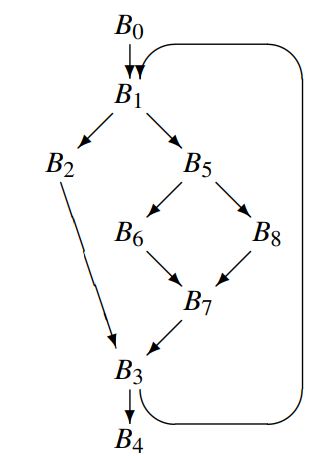
\includegraphics[scale=0.3]{images/r1.png}
\end{figure}

This information is usually represented as dominance sets for each node. A dominance set is defined as the set of all nodes that dominates the node $n$, which are found using the formula:

\[Dom(n)={n} \cup (\bigcap_{m \in preds(n)} Dom(m))\]

For completeness, here are the full dominance sets for the CFG above,

\begin{figure}[H]
  \centering
  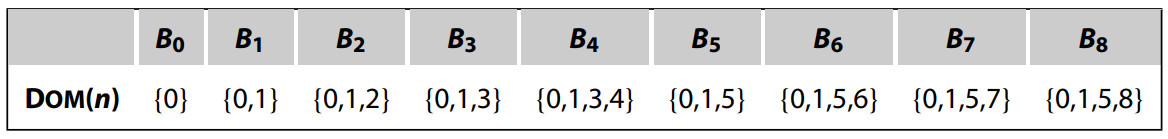
\includegraphics[scale=0.3]{images/r2.png}
\end{figure}

Dominance information is especially useful for understanding execution guarantees, because by definition, it is known if node $y$ is reached, node $x$, which dominates it, has been executed.
Intuitively I can see how this would be useful for optimizations like loop invariant code motion and and other similar transformations but will need to look more into it's other uses.
Next I read about the iterative algorithm for computing dominance and how it's proven to halt using the fact that $Dom(n)$ sets shrink monotonically throughout iteration and they have a lower and upper bound, $1 <= |Dom(n)| <= |N|$. 

After that, I looked into the differences between forward and backward data-flow problems. Forward data-flow problems are problems where information inherently "flows forwards" from the entry points to the exit point. An example of this that's easy to think about is constant propagation, values are computed while moving through the program and used in later blocks. Backward data-flow programs are a bit less intuitive, but encompasses problems like computing liveness information, so which variables are live at a certain point in the program. Basically, if a problem is defined in terms of predecessor basic blocks, then it is a forward data-flow problem and if it's defined in terms of successor basic blocks then it's backward data-flow. I also read about techniques that can be used for implementing them efficiently. For forward problems like dominance, the algorithm should use Reverse Postorder (RPO) on the normal CFG, while for backward problems like LiveOut, an RPO on the reversed CFG is needed. The reversal of the CFG creates a unique exit node if one does not exist.

There are also some precision issues that show up in data-flow analysis where invariants of the language aren't accurately represented in the analysis, some examples are unreachable successors when a loop condition is constant and imprecision when dealing with aggregate types like structs and arrays. Two loads/stores to an aggregate type may be disjoint, but traditional data-flow analysis will report them as aliasing, so extra work would need to be done. This imprecision can contribute to inefficiencies but is can be addressed through other optimizations and more advanced forms of analysis. Some other features that introduce extra complexity into analysis are pointers and function calls, especially with respect to aliasing and side-effects.

Liveness on an SSA (Static Single Assignment) representation was the next topic I read about, where liveness analysis is used to compute live-in/live-out sets at basic block boundaries. For register allocation, live ranges are derived by backward traversing instructions until a definition (def) is encountered. Something that I was initially confused about was the benefits of the differing granularity of liveness information and the different types of similar, but different, liveness information used in a compiler. Going into this chapter I had implemented the instruction-level liveness analysis, but not the basic-block version, so which seems like it strictly encodes more information and is seemingly better. This is not true though, instruction-level liveness isn't needed for most optimization passes and the live ranges it results in are more unwieldy to deal in general. Also, given one granularity, it is trivial to compute the other, so one is not strictly better or more powerful.

\subsection{Week 2: Static Single Assignment construction} 

This week I read chapters 5 and 9 of EC as well as chapter 3 of the SSA Book. First I read about benefits of keeping more invariants around after constructing the Intermediate Representation(IR), which is part of the motivation for Static Single Assignment form. One interesting example I came up with that I haven't seen before and takes advantage of high-level/source-level invariants would be with sorting and searching. If the compiler knows the semantics of sort it can potentially use the fact that all elements in a list are sorted until that list is modified. However, if the compiler was instead given lower-level IR that sorts a list it would be much harder to know what it's purpose is and use that info in the future.

\begin{lstlisting}
  li = list(...)
  li.sort()
  res = li.search(10) // we know li is sorted so this can use a binary search now
\end{lstlisting}

Next, I got a brief introduction to SSA form.
The big benefit of SSA form is that it encodes data-flow and control-flow directly into the IR,
no need to rerun separate data-flow analysis passes constantly, instead SSA will just need to be reconstructed if it is invalidated by a transformation.
Basically, SSA form allows the results of data and control flow analysis to be "shared" across many transformations.
A program is in SSA form when it meets two constraints: each definition has a distinct name and each use refers to a single definition.
This essentially means that each name/variable in SSA is a constant, so every time the name "a1" is referred to it will always have the same value unless it's definition is executed again, like during a loop.
To transform an IR into SSA form, $\phi$-functions must inserted at join points, which are blocks with multiple predecessors that effectively merge multiple control-flow paths.
Some other small complications, when a basic block with $\phi$-functions is entered, all of its $\phi$-functions must execute concurrently and before all other statements.
This is conceptually very similar to how function parameters work, which is why there is a variant of SSA, that uses "basic-block parameters", so parameters are passed when branching/jumping to a block,
mirroring how parameters are passed to a function, although with minor differences.

There are multiple different types of SSA I can construct, it's a tradeoff between speed,
implementation complexity, and "elegance" of the resulting SSA output.
There is a minor speed benefit for later passes to emitting less $\phi$ instructions, but in the end it is very small and constructing SSA form with less $\phi$ instructions takes longer to begin with.
Maximal SSA is the simplest to implement, at the start of each block with multiple predecessors, also known as a join point, a $\phi$ instruction,
$s = phi(\_,\_)$, is inserted for every name that the code either defines or uses in the current procedure.
Minimal SSA is when a $\phi$ instruction is inserted at any join point where two definitions for the same original name meet.
However, some of those $\phi$ instructions will be dead.
Pruned SSA is when a liveness test is added to the $\phi$-insertion algorithm so dead $\phi$-instruction are never added.
This means LiveOut sets, which were discussed last week, must be constructed which causes the cost of building pruned SSA to be higher.
Lastly, Semipruned SSA is conceptually between minimal SSA and pruned SSA.
Before inserting a $\phi$ instruction, the algorithm eliminates any names that are not live across a block boundary.
This reduces the number of $\phi$ instructions inserted without needing to compute LiveOut sets,
but as expected it can not omit as many $\phi$ instructions as pruned SSA.

There was also a brief section on SSA deconstruction, which needs to be done before attempting to generate machine code since $\phi$ instructions are not "real" instructions that a machine can execute.
First of all, a critical edge is an edge from a node with multiple successors to a node with multiple predecessors.
An easy way to do SSA deconstruction is just two steps, first split critical edges then for each phi instruction,
create a new SSA name $t_{i}$ and replace the $dest = \phi[{bb_{1},v_{1}}, {bb_{2},v_{2}}, \dots]$ with $mov dest, t_{i}$.
Then for each predecessor block insert a copy from the corresponding $\phi$ operands to that new name, b1: $mov t_{i}, v_{1}$, b2: $mov t_{i}, v_{2}$, etc.

Lastly, I wonder if there are other types of IR that make sharing other types of analysis between passes easier,
just like SSA does for data-flow?
The cost would be maintaining whatever invariants are required by it just like SSA has invariants that must be maintained,
like one definition for multiple uses.
Also, some other unrelated questions I will bring up during my weekly meeting:
What stage of the process should I insert critical edges?
What analysis/transformation would require it?
I can see if being useful for inserting moves/copies needed for SSA deconstruction, but I'm assuming other transformations would require it as well.

\subsection{Week 3: Register Allocation}

The chapters I read this week were 13 of EC as well as 21 and 22 of the SSA book.
Additionally, I also read a few papers that focused mainly on SSA deconstruction
\cite{ssadecon} and linear scan register allocation \cite{intervalsplitting}, \cite{lsrossa}.
I have implemented a basic version of linear scan register allocation already,
so I'm mainly looking for ways I can improve my implementation and make it more intuitive.

The first topics I read about described the old approaches to register allocation and how we ended up where we are today. Conceptually, what we refer to as register allocation today, can be split up into two separate problems. The first problem is just called register allocation where the goal is to map an unlimited set of virtual registers onto the more constrained register set of the target machine. The second problem is register assignment, which is mapping the set of allocated registers to the actual physical registers of the target machine. The register set is represented by register classes, some common examples would be general purpose registers(8/16/32/64-bit), floating point registers(Single/Double-precision), and flags. Additionally, converting between register classes may have a cost, so this can be modeled as well. Also, some register classes may overlap, like single and double-precision floating point numbers and different width general purpose registers which further complicates the implementation. 

One way I can split up my register allocation is by constructing a mapping of virtual registers to physical registers or stack slots. Then, I would have a separate step that rewrites the virtual registers to use physical registers and memory operations as well as inserting spill code where needed. This would make it easy, because the register allocator itself will not have to worry details related to spilling and storing/loading to memory, everything will just look like a virtual register.

Also, another important job of the register allocator is to manage spill code. Spill code refers to the  loads and stores to memory inserted by the register allocator when there are not enough registers on the target machine to directly represent the target program using the register allocation algorithm. The register allocator should aim to minimize the impacts of spill code because using memory incurs a much higher penalty than registers do. The three major points that must be managed are: execution time, code space, and data space occupied by the spilled values.

An interesting thought I had during this chapter is: can you spill a value in one register class to another one instead of defaulting to the stack? For example, if I need 4 general purpose values in a function and only have 3 registers, instead of spilling to memory can I spill to a floating-point register? Would it ever be worth it and would the cost similar or less than memory?

\subsection{Week 4: Basic Optimizations}

The chapters I read this week for 9 and 10 of EC.
It started off with a brief overview of various types of machine independent and dependent optimizations.
A few examples of machine-independent optimizations are:
local value numbering, inline substitution, and constant propagation.
Meanwhile some examples of machine-dependent optimizations are:
peephole optimization, instruction scheduling, register allocation, tree-height balancing, global code placement, and procedure placement.
Some optimizations can be machine-independent and/or machine-dependent,
like loop unrolling, which relies on machine-independent information such as loop overhead and machine-dependent information such as instruction scheduling.

The 5 main focuses of the remaining content of the chapter are eliminating useless and unreachable code(Dead Code Elimination), code motion(moving loop invariant computation out of a loop for example), specializing a computation(using context to rewrite multiply or divide as shift when valid), eliminating redundant computations(reuse a computed values instead of recomputing it), and enabling other transformations(canonicalization).

\begin{figure}[H]
  \centering
  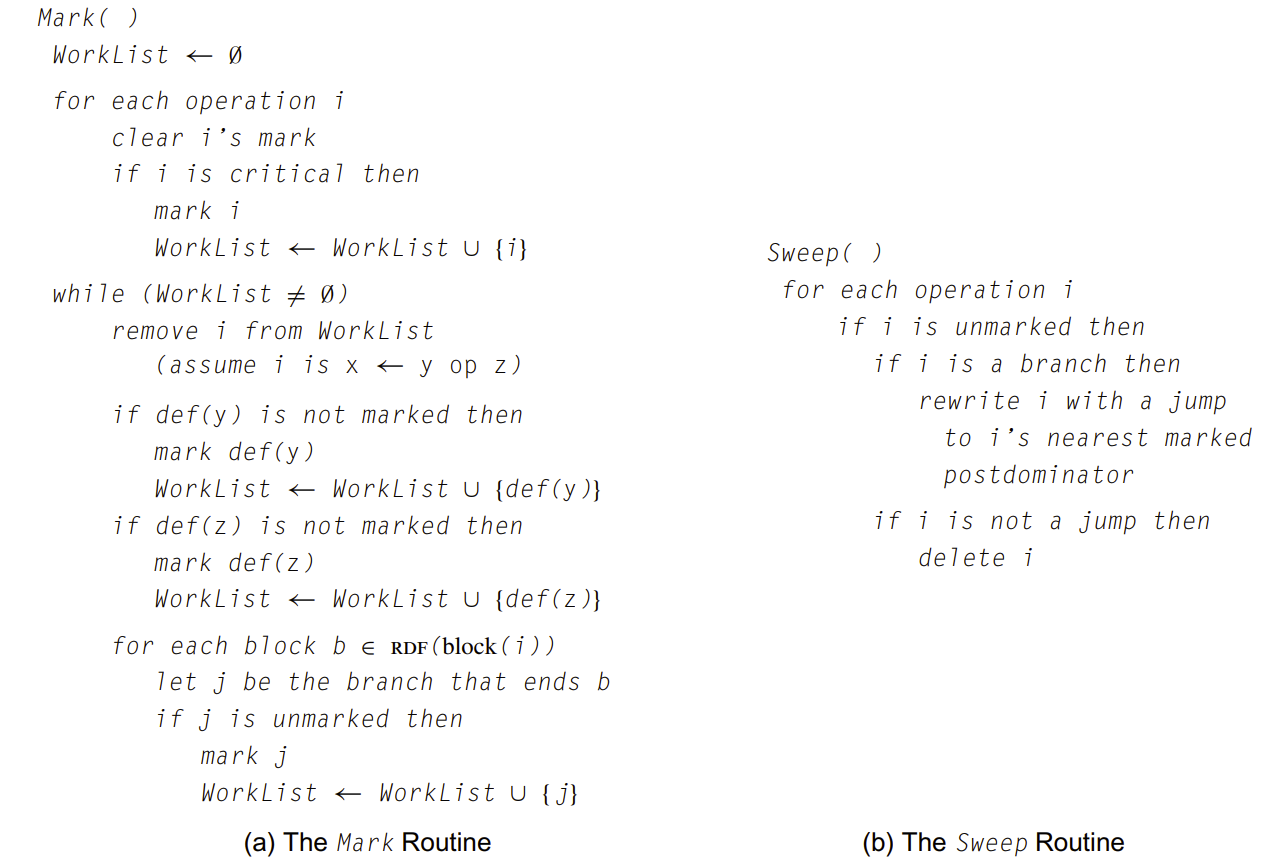
\includegraphics[scale=0.3]{images/r3.png}
\end{figure}

The next algorithm introduced by the book is a mark-sweep DCE algorithm using a worklist and relying on dominance information. This is more complicated than the naive approach to DCE, but allows removal of dead cycles in the graph, like would arise if a dead loop is present for example. The naive approach would just be removing blocks that have no valid incoming edges, but in the case of loops, the dead blocks would be keeping each other alive. This is also a problem that arises in during garbage collecting and reference counting as well, so, just like in this case, special handling is needed. It's interesting how similar problems show up in separate, but related, areas so often.

\begin{figure}[H]
  \centering
  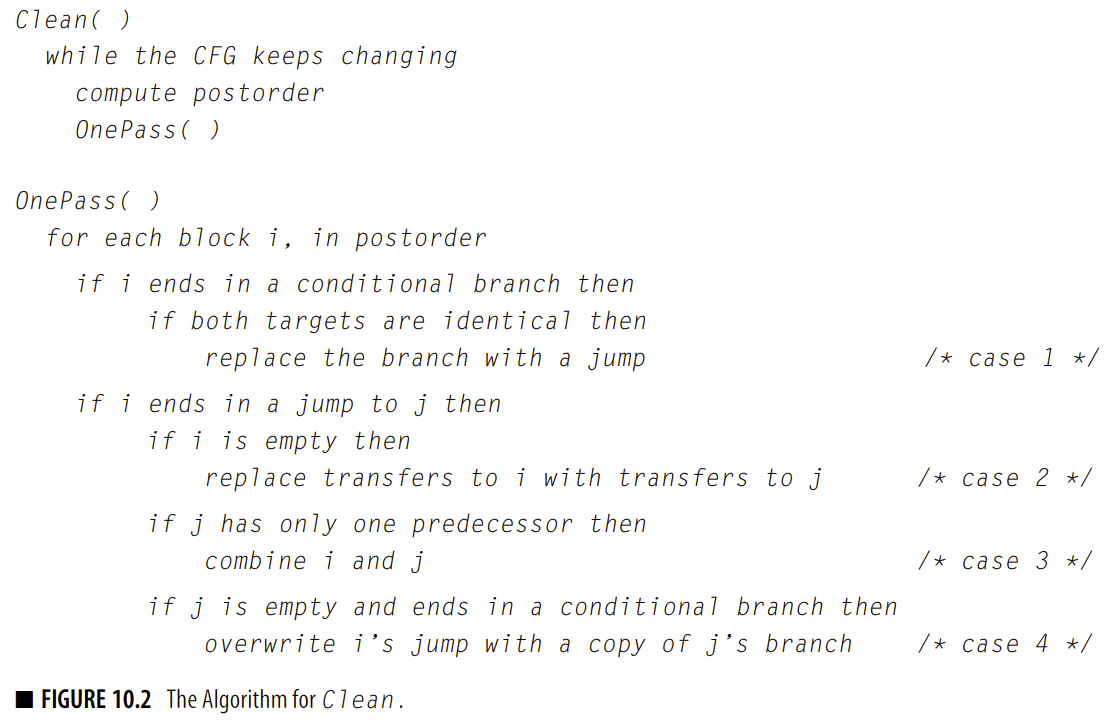
\includegraphics[scale=0.3]{images/r4.png}
\end{figure}

Next the book introduces an algorithm called "Clean". It's pretty common to mess up the CFG or leave unnecessary blocks and branches in it while doing optimization passes. This simplifies the implementation of those passes since they don't need to maintain an optimal CFG structure. The main use of "Clean" is to fix up these commonly left inefficiencies. The benefit is not only for performance, but also to simplify the CFG and reduce the number of cases other passes will have to dead with, which helps to enable more optimizations to run effectively. First, it folds redundant branches, so if both edges of a branch lead to the same block it will turn it into a single unconditional branch. Second, empty basic blocks are removed, so if a block only contains a jump, then merge it with it's successor. Third, basic blocks are combined, if a block has a single predecessor that unconditionally jumps to it then merge them. Lastly, branch hoisting, if multiple blocks unconditionally jump to a block with just a branch in it then the branch can be hoisted into each of the predecessors, which eliminates a jump.

\begin{figure}[H]
  \centering
  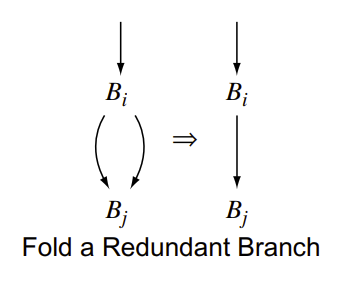
\includegraphics[scale=0.3]{images/r5.png}
  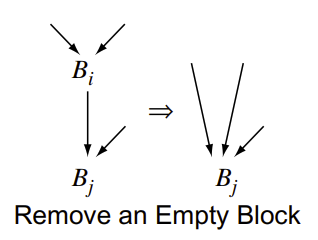
\includegraphics[scale=0.3]{images/r6.png}
  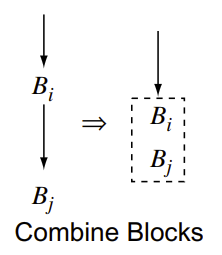
\includegraphics[scale=0.3]{images/r7.png}
  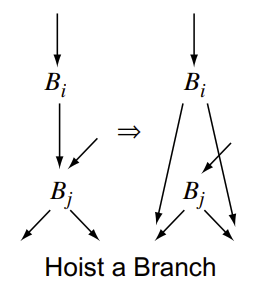
\includegraphics[scale=0.3]{images/r8.png}
\end{figure}

\begin{figure}[H]
  \centering
  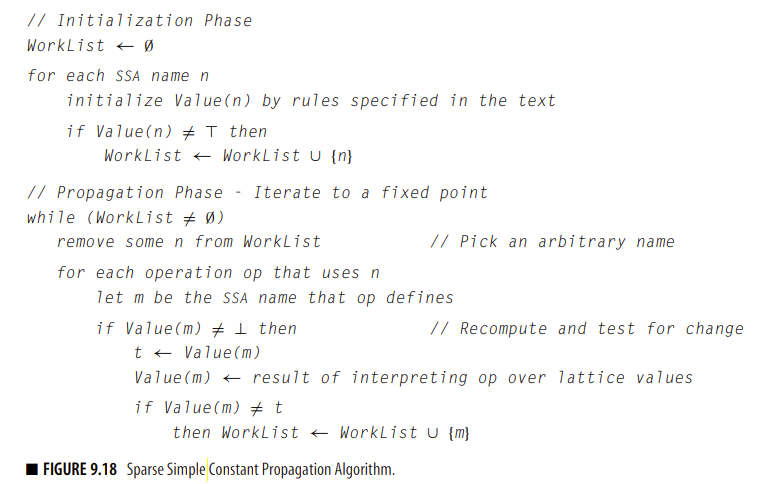
\includegraphics[scale=0.4]{images/r9.png}
\end{figure}

The next topic I read about was the Sparse Simple Constant Propagation (SSCP) algorithm. SSCP is distinct from an algorithm that is similarly named, but significantly more complicated, known as Sparse Conditional Constant Propagation (SCCP). The SSCP algorithm was also my first introduction to the concept of lattices and semilattices as well as the differences between pessimistic and optimistic aglorithms. For the SSCP algorithm, the compiler needs to annotate each SSA name with a value, and the set of possible values forms a semilattice.

In SSCP, semilattices are used both to initialize information about each name and to propagate information throughout the program.
The semilattice structure for this problem allows us to determine whether the value assigned to a name is a known constant.
Initially, $\top$ represents that we know nothing about the value of the name yet and need more information to make a determination,
conversely $\bot$ represents that the value cannot ever be determined.
As a result of the formulation of a semilattice, names can only move downwards in the lattice,
so their states can only change twice: first from $\top$ to a constant value, and then, if necessary,
from a constant to $\bot$.
After states are assigned to each SSA name, any value that has a constant state can be replaced directly,
while values with a $\bot$ state are known to change, meaning they cannot be replaced by a constant.
An important advantage of SSCP comes from Static Single Assignment (SSA) form.
In constant propagation without SSA, iterative analysis would need to account for blocks,
tracking constants as they flow in and out while intersecting values for names assigned multiple times.
The SSA form simplifies this process significantly since each SSA name is assigned exactly once.
SSCP is an optimistic algorithm, it assumes that all values can be constant (by initializing to $\top$) and waits for additional information to prove it otherwise.
Contrasted with a pessimistic algorithms, which in this case, would be the equivalent of assuming no values are constant and requiring information that proves the opposite.

\subsection{Week 5: Sparse Conditional Constant Propagation (SCCP)}

This week I learned about Sparse Conditional Constant Propagation (SCCP),
which is an optimization that combines constant propagation and dead code elimination (DCE) to achieve results that are not possible by running these optimizations separately.
SCCP propagates value and reachability information at the same time throughout the CFG.
The interdependence between constant propagation and DCE is what makes SCCP extra effective.
Removing unreachable code exposes more constant values, and at the same time propagating constants can identify previously unknown unreachable blocks.
One way SCCP is more powerful is because of how it handles branching on constants.
Unreachable code paths are ignored and branch-specific invariants, such as a value known to be $<1$ as a result of the branch condition,
are used to find more constant values later in the CFG. Also, CFG edges can be eliminated more often.
It can be determined which branches of a conditional statement are taken and remove CFG edges associated with untaken branches.
Lastly, unreachable operations can be handled in a way that doesn't inhibit finding constants in the future.
SSA definitions in unreachable blocks are set to $\top$, so those operations can be ignored unless their blocks become reachable.

The benefit seen from combining optimizations into SCCP raises some questions , such as what are some other optimizations that benefit from being combined? Also, what properties do separate optimizations need to have in order for combining them to be beneficial? The answer seems to be that they need to be interdependent.

I also explored Operator Strength Reduction (OSR) and other related loop optimizations. To begin with, a region constant is a value that remains unchanged throughout the iterations of a loop, while an induction variable is a value that consistently increases or decreases by a fixed amount in each iteration. A variable is a a region constant if it is defined by an immediate operation or if its basic block dominates the header block of a loop, which is where the induction variable is initialized. An example of a case OSR can optimize occurs when an induction variable is used in a multiplication operation with a region constant, the multiplication can then be replaced with repeated addition, which results in the same results and has better performance. Similar transformation can be done for other operations as well, such as division.

\subsection{Week 6: Value Numbering and Redundancy}

It is common to have a peephole or pattern-matching pass which canonicalize expressions, and enables future optimizations by ensuring they don't need to handle potentially infinite representations of computations that have identical results.
For instance, trivial expressions like \textit{a = imul c, 0} can be replaced with \textit{a = mov 0}.
It's easy to handle this once rather than in every single pass that could potentially check if a specific value is a constant $0$.
These transformations can also be integrated directly into constant folding or GVN hashing, but I find it cleaner to have a smaller separate pass that can be run instead of needing to run an entire large optimization pass. 

\begin{figure}[H]
  \centering
  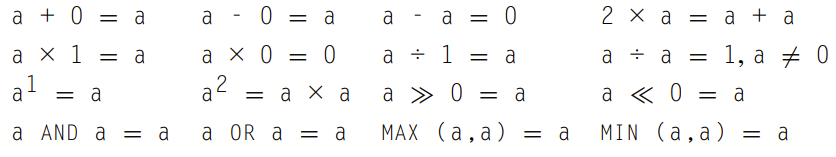
\includegraphics[scale=0.4]{images/r10.png}
\end{figure}

More complex cases, such as deducing equivalence between two SSA (Static Single Assignment) names through present challenges.
This requires a pass called Global Value Numbering (GVN), which identifies redundancies either through syntax-driven (lexical equivalence) or value-driven (proving equivalence) methods.
GVN relies on hashing expression trees recursively, with internal nodes hashed by operator and operand value numbers.
SSA simplifies extending local value numbering to GVN, $\phi$ instructions complicate the process, requiring graph traversal in reverse postorder of the dominator tree to make sure all opeands are available when a $\phi$ is reached.

Here is a fast algorithm for constructing a dominator tree as well, which will be useful when implementing the dominance-based version of GVN.

\begin{figure}[H]
  \centering
  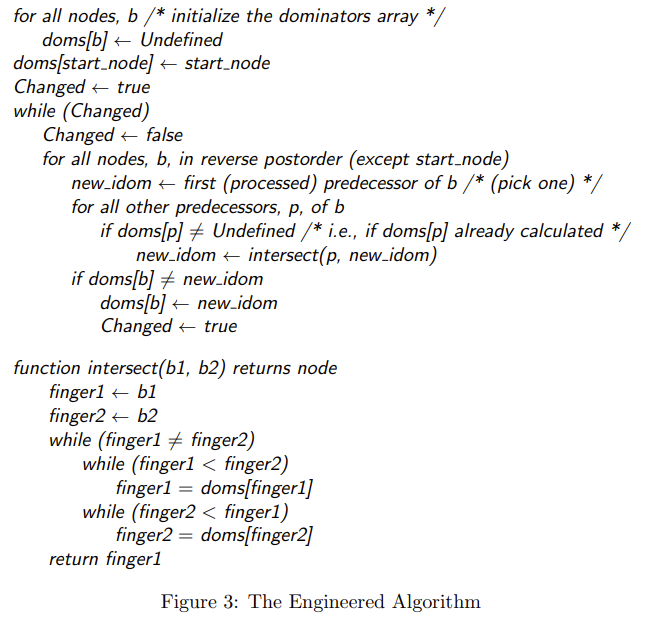
\includegraphics[scale=0.45]{images/r11.png}
\end{figure}

\subsection{Week 7: Instruction Selection/Scheduling}

Instruction selection (ISEL) and scheduling are important tasks in a compiler backend, translating intermediate representations (IR) to machine instructions while optimizing for performance. Two common ISEL strategies are tree-pattern matching and peephole optimization. Tree-pattern matching operates on a high-level tree-based IR, generating target instructions by matching subtrees with predefined patterns. Peephole optimization, in contrast, works on a linear low-level IR, applying rules within a sliding window of instructions to improve the code.

More general, non-hardcoded, instruction selectors use separate IRs to represent patterns that should be matched. They enable optimizations like folding address calculations into load/store operations or combining memory access with arithmetic to be done easier. For example, multiple IR instructions representing address calculations and loads might be merged into a single x86 instruction such as \textit{add rax, QWORD [rsp+rax+0x48]}. 

\begin{figure}[H]
  \centering
  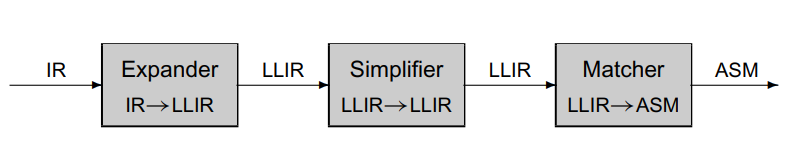
\includegraphics[scale=0.4]{images/r12.png}
\end{figure}

Instruction scheduling arranges operations to maximize processor resource utilization. Common techniques include list scheduling, a greedy heuristic algorithm that schedules operations based on their dependencies and priorities. The dependency graph, which represents data flow and operation latencies, guides this process by ensuring each operation executes only when its operands are available. Critical paths in the graph represent the minimum execution time for a block of code, while scheduling strategies aim to reduce stalls and maximize throughput.

\begin{figure}[H]
  \centering
  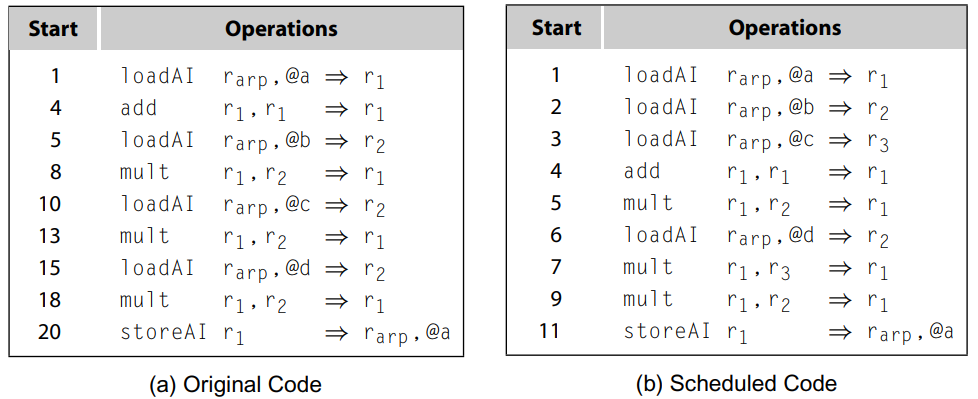
\includegraphics[scale=0.4]{images/r13.png}
\end{figure}

Another related optimization is basic-block scheduling, this optimizes block layouts by choosing which successor block in a branch becomes the fallthrough block, and other strategies for minimizing jumps for faster execution.

\subsection{Week 8: Loop Optimizations}

Lazy Code Motion (LCM) is a compiler optimization that performs loop-invariant code motion while also eliminating fully and partially redundant computations. The goal is to move computations to locations in the program that are executed less frequently. Redundant computations occur along all execution paths, and partially redundant ones occur on only some paths.

\begin{figure}[H]
  \centering
  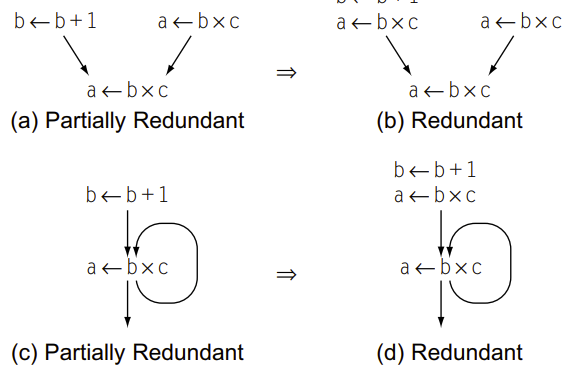
\includegraphics[scale=0.4]{images/r14.png}
\end{figure}

LCM computes sets of "available" and "anticipable" expressions. An available expression is one that has already been computed on all paths entering a basic block, while an anticipable expression is one that will be computed on all paths leaving a point in the CFG. These sets are used to derive the "earliest" legal placement of computations, which represents the earliest CFG edge where an expression can be safely inserted. Additionally, LCM determines "later placements" that allow computations to be delayed which can help minimize the lifetimes of computed values.

Earliest placement: Based on available and anticipable expressions, it identifies the earliest edge where a computation can legally occur. Critical edges may need to be split to enable safe placement. 

\[Earliest(i, j) = AntIn(j) \cap \overline{AvailOut(i)} \cap (ExprKill(i) \cup \overline{AntOut(i)})\]

\begin{figure}[H]
  \centering
  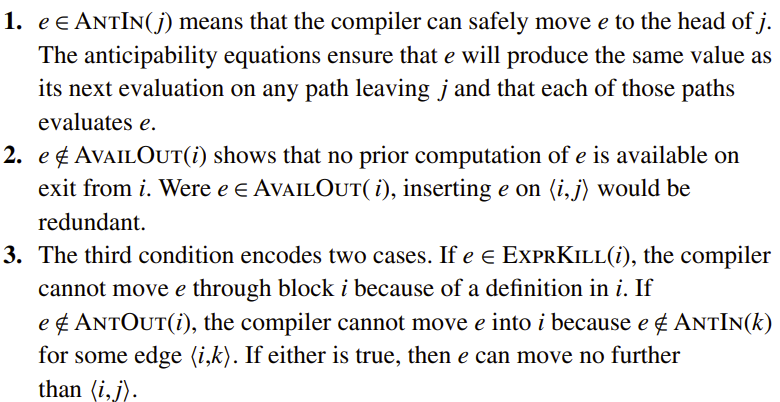
\includegraphics[scale=0.4]{images/r15.png}
\end{figure}

Later placement: Defines the latest CFG edge where a computation can still have the same effect. This is determined using the LATERIN and LATER sets, which track expressions that can be safely moved across edges or nodes without altering program behavior.

\[LaterIn(j) = \bigcap_{i \in pred(j)} Later(i,j), j \neq n_{0}\]

\[Later(i,j) = Earliest(i, j) \cup (LaterIn(i) \cap \overline{UEExpr(i)}), i \in pred(j)\]

Finally, LCM calculates the insert and delete sets, which specify where new computations should be inserted and where redundant computations should be removed. Insertions occur at the end of a source block or the start of a target block, depending on the CFG structure.

\[Insert(i,j)=Later(i,j) \cap \overline{LaterIn(j)}\]

\[Delete(i)=UEExpr(i) \cap \overline{LaterIn(i)}, i \neq n_{0}\]

This performs hoisting as well, which reduces duplication by moving computations out of branches into their parent block.
If an expression is anticipable at the end of a block, it can be moved to that point.

\subsection{Week 9: Function Optimizations}

Functions form boundaries in the code, it keeps the amount of code that has to be dealt with at a time small, which makes compilation faster and compile-time data structures smaller. However, these boundaries also limit optimizations across functions and introduce extra costs, such as the need for prologue and epilogue sequences. Inline substitution, which replaces a function call with a rewritten copy of the callee’s body, eliminates the overhead associated with function calls, including allocating an activation record, evaluating parameters, preserving the caller's state, creating the callee’s environment, transferring control, and returning values. By removing these boundaries, inlining allows the compiler to leverage invariants previously inaccessible and apply additional optimizations, such as sparse conditional constant propagation (SSCP) or dead code elimination (DCE), when function parameters are constant. Inlining operates on a program’s call graph, as opposed to the control flow graph (CFG) used in many other optimizations, and involves two main challenges: determining which call sites to inline and performing the inlining transformation. Despite its benefits, inlining can degrade performance by increasing code size, reducing the effectiveness of other optimizations, and increasing register demand and pressure.

At each call site a decision must be made whether or not to inline. However, this decision has an effect on all other call sites that interact with the current function, since it changes the characteristics of the function. This means, after inlining at a call site, the "cost" of inlining the current function may increase enough that it is no longer inlining it into it's callers. Therefore, the order that call sites are inlined has an effect on the outcome, heuristics must take this into account. Some criteria for deciding whether a function should be inlined or not: callee size, caller size, constant-valued parameters(may enable SSCP and DCE), static call count(low static call count is a good candidate), frequently called or not(if it's in a nested loop), and if it's a leaf function.

\subsection{Week 10: Equality Saturation}

Traditional optimization techniques in compilers suffer from the phase ordering problem and rely on local profitability heuristics, so only the short-term impact of transformations is considered instead of the long-term impact.
Equality saturation is exploring a space of equivalent programs instead of following a single optimization path.
This global approach enables finding an optimal solution by deferring profitability decisions until the entire space has been explored.

The Program Expression Graph (PEG) non-destructively represents many equivalent computations simultaneously.
The process involves converting a Control Flow Graph (CFG) into a PEG, applying rewrite rules to explore equivalences, and finally converting the optimized PEG back into a CFG.
This helps to mitigate the phase-ordering issue and allows a more efficient exploration of the optimization space.
It is also able to leverage global profitability heuristics instead of local, so transformations that are unprofitable initially can be explored and may yield better results later.

For example, a multiplication by 4 can exist at the same time with its equivalent left-shift operation in the PEG.
This flexibility enables algebraic simplifications, constant propagation, and strength reductions, among other optimizations.
However, it currently struggles with certain transformations, such as loop unrolling, which depend on control flow.
Equality saturation also enables emergent optimizations that would not have been found as a result, since multiple forms of equivalent operations are represented without destroying the previous version. 

Aegraphs address some performance issues and as a result are more practical to use for real-world compilers.
Traditional e-graphs, can easily represent bidirectional rules such as commutativity and associativity rules,
but aegraphs use directional rewrites.
The pipeline is streamlined into three linear passes: build and rewrite, extraction, and scoped elaboration.

Scoped elaboration can handle code motion and redundancy elimination across basic blocks as well. This can subsume traditional optimizations like Global Value Numbering (GVN), Loop-Invariant Code Motion (LICM), and rematerialization.

\subsection{Week 11: LLVM}

This week I looked into deep learning (DL) compiler architecture first, then moved on to LLVM and GHC.

First, looking at DL compilers.
In this context, high-level IR often refers to the computation graph,
it is a hardware-agnostic representation that simplifies optimization.
Computations are represented as directed acyclic graphs (DAGs),
where nodes signify DL operators (e.g., convolution, pooling), and edges denote tensors.
However, traditional DAG-based representations can suffer from semantic ambiguity due to undefined computation scopes.
To address this, let-binding is introduced, as seen in TVM's Relay IR, which combines DAG structures with scoped functions.

There are a few approaches for representing tensor computation:
First, function-based methods, like XLA's HLO, encapsulate operations across multiple levels (program, function, operation).
Second, lambda expressions bind variables to computation rules, which is used by TVM, where tensor expressions are defined using output shapes and lambda functions.

Data representation varies as well.
Some common representations are placeholders (explicit shapes),
unknown shape representations (dynamic dimensions), and memory layouts (tiling, padding, striding).
Operators provide functionality, such as broadcasting for shape compatibility,
control flow representation for dynamic models, and derivative computation for gradient-based learning.

Now looking at optimization pipelines, these include both frontend and backend passes.
For the frontend frontend, optimizations work on the computation graph,
this includes node-level simplifications (like removing no-ops),
block-level operator fusion, and global optimizations like static memory planning.
Backend optimizations focus on hardware-specific issues, this includes memory allocation and loop transformations,
which play a big role in GPU-based compilation as compared to CPU compilation.
Techniques like loop fusion, tiling, and unrolling improve locality and parallelism.

\begin{figure}[H]
  \centering
  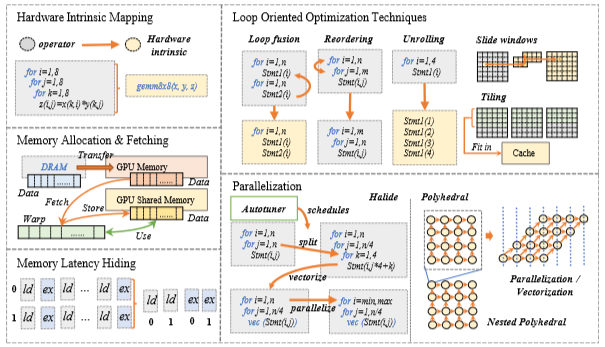
\includegraphics[scale=0.4]{images/r16.png}
\end{figure}

Lastly, LLVM and other backend frameworks streamline code generation by providing reusable components for target-specific optimizations.
LLVM's architecture is designed to be madular and has extensible passes and pattern-matching interfaces.
GHC has similar goals.
It has a more minimalistic Core IR as opposed to LLVM's IR.
It also has rewrite rules and a modular pipeline for defining domain-specific transformations which is even easier to extend than LLVM.

\subsection{Week 12: Profile-Guided Optimization (PGO)}

The first topic I read about this week was Profile-Guided Optimization (PGO). PGO is a compiler optimization that uses runtime profile information to improve the performance of a program. The process involves three main phases: instrumentation, training, and optimization. During the instrumentation phase, probe instructions are added to an intermediate representation of the program. In the training phase, the instrumented executable is run on representative workloads to collect profile data, which is critical for success. Using unrepresentative workloads can negatively affect performance, especially for complex software like web browsers. Finally, in the optimization phase, the collected profile data informs decisions such as function inlining, branch optimization, basic block reordering, and determining whether to optimize functions for speed or size. Frequently executed functions might be optimized for speed, while infrequently used ones are optimized for size.

Recent work in PGO includes using machine learning models to infer branch probabilities as a supplement to existing branch prediction heuristics. These models, such as ensembles of boosted decision trees, leverage branch profile data from tools like LLVM. While they improve branch prediction accuracy, they lack the workload-specific advantages of traditional PGO.

The next topic I read about was the polyhedral model. The polyhedral model is a mathematical framework for loop transformations, particularly in optimizing nested loops for parallelism and locality. It represents iteration domains and dependencies as geometric objects and schedules computations based on affine transformations. For instance, two loops producing different schedules can violate dependencies if the transformation changes the execution order of dependent statements. The model analyzes dependencies and checking that they remain unbroken under the new schedule. For example, reversing a loop’s execution order might violate data dependencies if a later statement reads data produced by an earlier one in the original order. The legality of a transformation is determined by solving systems of constraints derived from dependencies.

\begin{figure}[H]
  \centering
  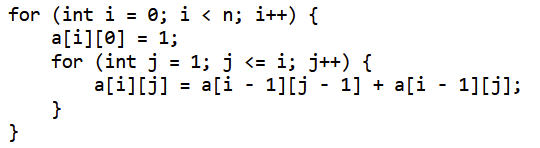
\includegraphics[scale=0.4]{images/r18.png}
  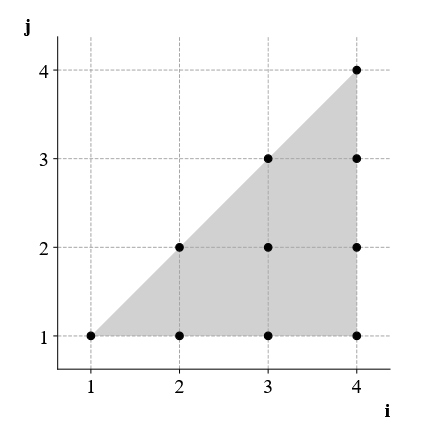
\includegraphics[scale=0.4]{images/r19.png}
\end{figure}

The main steps of polyhedral optimization include extraction of the iteration domain, dependence analysis, scheduling to compute an optimized execution order, and AST generation to produce executable code from the new schedule. Optimizations like loop fusion can be done by defining affine functions for schedules and solving constraints using tools like SAT solvers.

\begin{figure}[H]
  \centering
  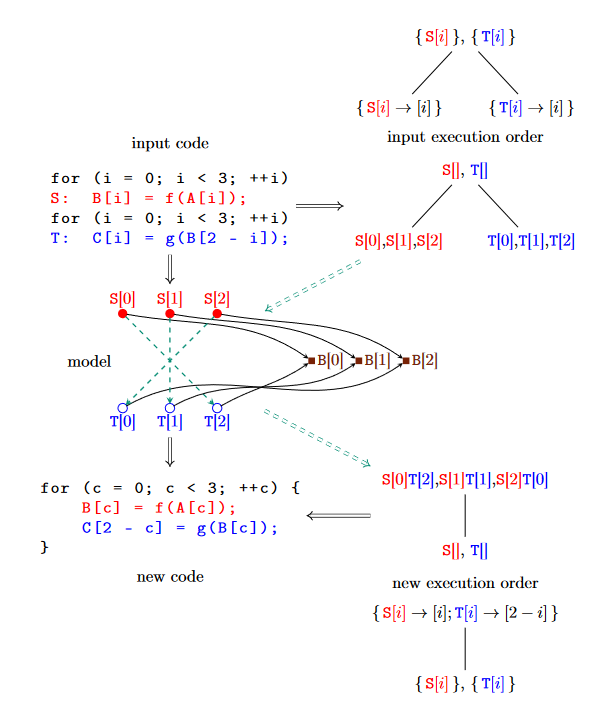
\includegraphics[scale=0.4]{images/r20.png}
\end{figure}

\subsection{Week 13: Sea of Nodes (SoN) and RVSDG }

First, I read about Sea of Nodes(SoN). SoN is a graph-based intermediate representation (IR) designed for Just-In-Time (JIT) compilers, use-def chains and SSA are a core component and built directly into the IR. Nodes represent operations, while edges denote dependencies, either control or data. Control flow is replaced by REGION nodes, which merge control values from predecessors, this effectively unifies control and data dependencies into a single structure. Removing optional control edges can enable better global optimizations but would complicate serialization in the process. The execution model uses a Petri Net for the control graph, where a control token traverses nodes like START, REGION, and IF, and a data subgraph, where data flows along edges.

Thick edges are control, thin are data, and dashed edges are optional control edges that show which region a node belongs to.

\begin{figure}[H]
  \centering
  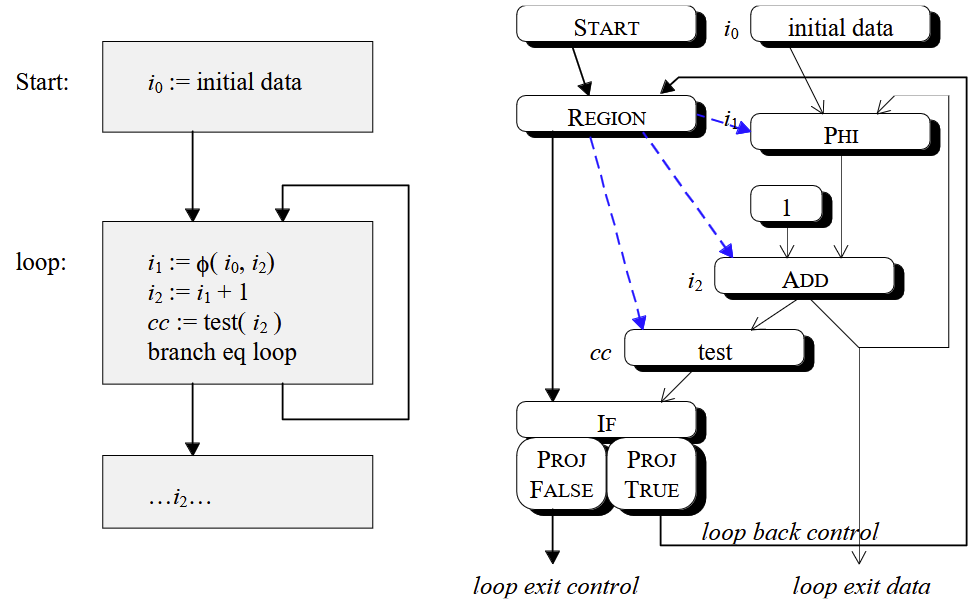
\includegraphics[scale=0.4]{images/r21.png}
\end{figure}

SoN is able to do optimizations at parse-time by doing peephole/local optimizations directly while constructing the IR. These parse-time optimizations, like constant folding and local common subexpression elimination, have a limited scope because assumptions can not be made about unparsed code. Also, SoN allows and relies on optimizations like global code motion (GCM) to properly schedule nodes. Memory and I/O are treated as global states that are modified through STORE/LOAD nodes. This allows reordering of operations between operations that must be properly ordered (like memory/IO operations).

\begin{figure}[H]
  \centering
  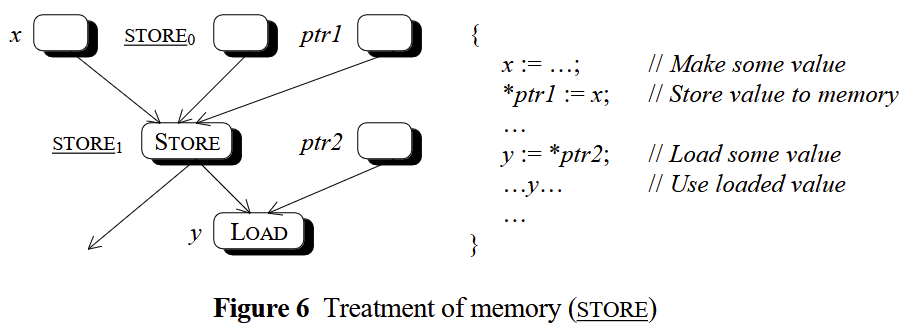
\includegraphics[scale=0.4]{images/r22.png}
\end{figure}

RVSDG is a hierarchical, acyclic graph that prioritizes data dependencies over control flow, so it is especially good at data-centric optimizations and parallelism. Nodes represent computations, and edges encode dependencies, with structural nodes (e.g., Theta for loops, Gamma for conditionals) explicitly representing program constructs. This IR enforces strict SSA form, so there is no need for expensive analysis passes such as SSA reconstruction or loop detection to be rerun constantly, which are common in CFG-based approaches like LLVM.

RVSDG has built in normalization, so programs that differ only in the sequence of independent operations will more share the same representation, this is unlike a CFG-based approach which has an explicit ordering. This lack of ordering helps to enable more optimizations, such as loop-invariant code motion, without requiring extra passes. Stateful computations are ordered through state edges, this preserves correct execution order without enforcing an arbitrary order for independent computations as well.

\begin{figure}[H]
  \centering
  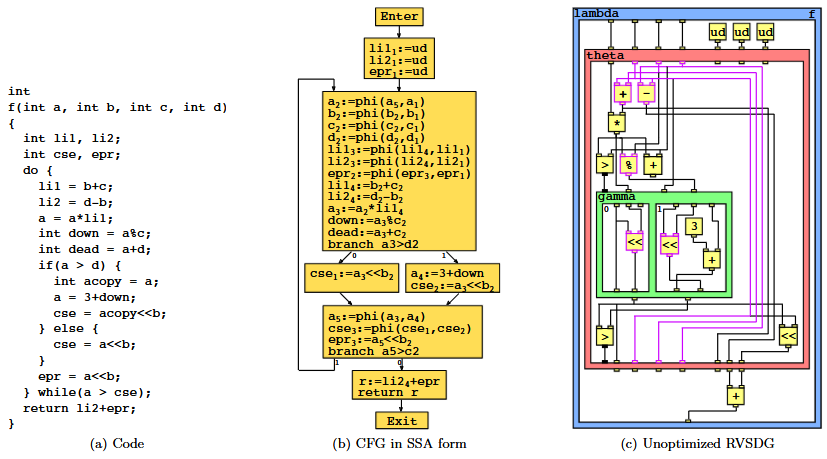
\includegraphics[scale=0.4]{images/r23.png}
\end{figure}

This IR also helps to avoid the loss of semantic information and invariants present during early compilation stages. For example, in C++, the contents of two distinct std::vector instances can never alias by language semantics, this is able to be represented properly in RVSDG since vector contents will be modeled as independent states from the very beginning.

\subsection{Week 14: Phase Ordering }

This week I read the paper Mitigating the Compiler Optimization Phase-Ordering Problem Using Machine Learning.

Modern compilers apply a fixed set of optimizations across all functions regardless of their content. As an example, GCC includes around 250 optimization passes, but only a subset is applied by default and in a fixed order. This approach ignores the potential performance gains of choosing a specific set and order of optimizations for each function individually. Choosing the optimal ordering of optimizations is known as the phase-ordering problem. Previously, this is an area where genetic algorithms (GAs) are commonly used, but they are computationally expensive which makes them mostly impractical to use in the real-world. In this paper they propose an alternative approach using Neuro-Evolution of Augmenting Topologies (NEAT). Using NEAT would shift the computational cost from runtime to train-time, and it would hopefully still give performance benefits similar to GAs. For simplicity, and because of the unpredictable nature of the effects of optimizations, the authors use NEAT for predicting the most beneficial optimization at each step instead of generating a sequence of optimizations upfront. Interestingly, the authors state the optimization problem has the Markov Property, which means only the current state (features) matter when determining the next optimization to apply. Although, intuitively, I would assume there would be a benefit to long term planning.

The phase-ordering problem requires finding the optimal order of optimizations for maximum performance. Although GAs are effective at discovering beneficial sequences, their high computational cost limits practicality, especially in Just-In-Time (JIT) compilation scenarios. Instead, this work adopts a machine learning approach using NEAT to train an artificial neural network (ANN) to predict the best optimization at each stage. This shifts the computational cost to training, allowing fast inference during compilation.

First they did feature extraction, which had the goal of representing the most relevant characteristics  of each function needed to inform optimizations. Then, they had to search for an ANN using NEAT, so a population of 60 networks is generated, then the top 10 performers from each generation are kept, which is then repeated. At each step mutation and crossover operations are used to evolve the network structures. Lastly, the final trained ANN is used to predict probabilities for each optimization pass based on the extracted features. This is ran multiple times in succession until it gives the stop signal.

The resulting performance was decent. In adaptive mode(dynamically choose optimization levels), they achieved an average runtime speedup of $8\%$ and a $4\%$ improvement in total execution time compared to Jikes RVM's default adaptive mode. In non-adaptive mode(all functions compiled at highest optimization level), they improved runtime by an average of $8.2\%$ and total execution time by over $6\%$.
GA on the other hand, can theoretically find better optimization orders given unlimited time, but the NEAT approach gives good performance in a context where runtime speed matters.

The NEAT approach was effective for applications with a relatively flat profile, so a large number of functions shared the execution time. However, GAs still outperform NEAT when programs had very hot functions, where focusing on optimal ordering for just the high-impact functions instead of the whole program would give a larger benefit. There were also some challenges, such as potential infinite loops from when the predicted optimization does not change the features, which will cause it to give the same prediction again so it could give worse performance than a fixed optimization order in that case.

In conclusion, this paper introduced the NEAT approach as a practical alternative to GAs to mitigate the phase-ordering problem, especially in JIT compilers where runtime is very important. Execution time improvements reached up to $20\%$ in some cases.
Future work includes using this approach in Ahead-of-Time(AOT) compilers and adding profile data into the set of features used for prediction.

\pagebreak
\section{Implementation}

\subsection{Week 1}

The implementation activity for this week was liveness analysis.
I have previously implemented a version of liveness analysis that computed live ranges for each variable,
but the type of liveness analysis I will implement this week is on the basic-block level.
In other words, the LiveIn and LiveOut sets for each basic block in a function.

I took the following example above from Engineering a Compiler and modified it to be slightly more interesting.

\begin{figure}[H]
  \centering
  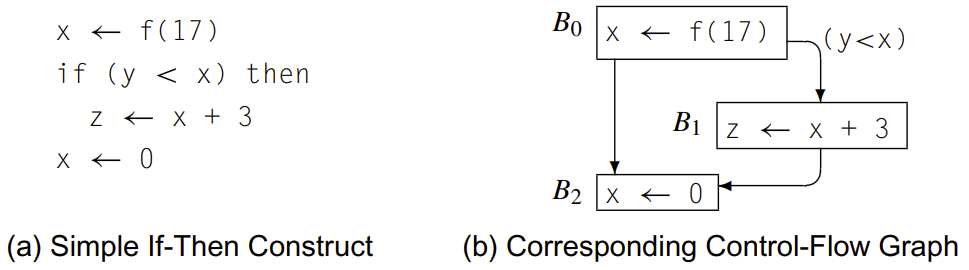
\includegraphics[scale=0.3]{images/i1.png}
\end{figure}

Here is the slightly modified version in C.

\begin{lstlisting}
int main() {
  int x = 17;
  int y = 6;
  int z = 0;
  if(y < x)
    z = x + y;
  return z + x;
}
\end{lstlisting}

Here is the C code translated to equivalent JBIR.

\begin{lstlisting}
  [win64]
  fn main() %0:i32
  entry:
    %1 = id 17.i32
    %2 = id 6.i32
    %3 = id 0.i32
    %4 = lt %2, %3
    brz %4 then cont
  then:
    %5 = iadd %1, %2
    br cont
  cont:
    %6 = phi [entry, %3], [then, %5]
    %7 = iadd %6, %1
    ret %7
\end{lstlisting}

Lastly, these are the liveness analysis results:

\begin{lstlisting}
entry:
  livein:
  liveout: 3 1 2

then:
  livein: 1 2
  liveout: 5 1 3

cont:
  livein: 1 3 5
  liveout:
\end{lstlisting}

Also, there was some work done on general infrastructure.

First, I started working on omitting the base pointer in generated x86\_64 code.
This is mostly done as an optimization on linux but windows has some special rules and it's done by default when using the Microsoft C Compiler (MSVC), even in debug mode.
There is also a requirement of a 40 byte shadow space for non-leaf functions which I have an initial implementation of as well.

Second, I added a new JBIR instruction, the "id" instruction. This is the identity operation and just puts it's operand in a virtual register. This was needed to make creating test cases easier, it shouldn't be used in normal code. It will also most likely be generated during register allocation in the future.

Additionally, I made a note of areas of the compiler I can improve on in future weeks that would make implementing future transformations and analyses easier:
First, while working on the original algorithm from Engineering a Compiler I realized a potential spot for improvement.
My implementation of control flow graph traversal is not ideal.
In EC there is a specific way they recommend traversing the CFG for forward/backward data-flow problems.
For forward data-flow the traversal should be Reverse Postorder (RPO) on the CFG and for backward data-flow RPO on a reverse CFG should be used.
It may be helpful to make a general CFG traversal that can be reused for different types of analysis/optimization.
Second, I assume basic blocks are in RPO in multiple places.
It would be a good idea to explicitly order them instead of depending on the frontend.
(Can also verify SSA)
Third, I assume the last block in a function is a unique exit node.
This constraint is never verified though and relies on the frontend behaving correctly.
I create a unique entry/exit node in the x86\_64 backend in order for stack frame creation/cleanup to work but don't do it in JBIR so it would be beneficial to add.
Fourth, I should consider properly implementing def-use/use-def chains in the future.
Currently I take advantage of them to compute live-ranges during register allocation but there is no existing general implementation that I can reuse yet.
Lastly, the way I manage analysis/optimization passes should be more organized especially if I'm planning on adding a bunch of them.
This is where a pass manager of would be very helpful.

\subsection{Week 2} 
The implementation activity this week was memory to register promotion, often referred to as Mem2Reg. Mem2Reg is basically a version of an SSA construction algorithm, but where the non-SSA variables are memory locations on the stack instead of normal named variables in the IR.

I only considered stack\_store/stack\_load chains for stack slots to be valid for promotion.
I could have expanded this to normal memory accesses with store/load, but this would have been an unnecessary complication.
As a result of compiling from C, the programmer is allowed to do arbitrary computation with pointers, so to sidestep this complexity for now if the address of a stack slot is ever used in a instruction other than a store/load,
then it is no longer valid for promotion.
An example of something that would cause this would be taking the address of a local variable in C then doing pointer arithmetic.
Some additional details, stack\_loads that are in the same basic block as their corresponding stack\_store can be elided completely.
A similar situation is basic blocks with one predecessor, loads in those can also be easily elided.
However, loads in basic blocks with two or more predecessors need to be replaced with phi instructions.
To do this, every time a valid load with those properties is encountered, it's predecessors are traversed until a corresponding store is reached along each path.
In other words, if a block has two predecessors then a store must be reached by traversals starting with each of them.
The final step is removing the dead stack slots.
Dead slots are kept track of throughout the load/store replacement step and are turned into no-ops.
This algorithm is what I implemented, and it seems correct at first glance, but it runs into issues with values that were used in a basic block dominated by a join point instead of the join point itself not getting the proper phi node inserted at that join point,
which were pointed out during a meeting, and I plan to fix in a future week.
Modern fast SSA construction algorithms use dominance frontiers for this, which not only would be more efficient, but would also fix the correctness issues present as well.

Here is some example IR.

\begin{lstlisting}
fn main() %0:i32
entry:
    %1 = slot i32
    stack_store %1, 100.i8
    brnz 1.i32 first second
first:
    br last
second:
    stack_store %1, 42.i8
    br last
last:
    %4 = stack_load %1 i32
    ret %4
\end{lstlisting}

This is the data structure that is built for each stack\_load.
The stack\_stores that correspond to each stack\_load and the basic blocks they are in is recorded.

\begin{lstlisting}
  %4 = stack_load %1 i32
  --------------------
  first: stack_store %1, 100.i8
  second: stack_store %1, 42.i8
\end{lstlisting}

Then the transformation is done, replace stores with the definition of an SSA name, loads with the use of an SSA name, and slots with a noop. 

\begin{lstlisting}
  fn main() %0:i32
  entry:
      noop
      %1000 = id 100.i8
      brnz 1.i32 first second
  first:
      br last
  second:
      %1001 = id 42.i8
      br last
  last:
      %4 = phi [first, %1000], [second, %1001]
      ret %4
\end{lstlisting}

I also made sure to keep track of areas to improve in future weeks.
First, improve SSA value/reg naming, maybe keep track of the next available name module-wide or function-wide,
instead of hoping there are no collisions.
This can possibly be built directly into the IR such that there are no explicit names,
just def-use chains, which is common in some more modern IRs.
Second, keep track of visited nodes when doing traversal,
at the moment it's very easy to get stuck in an endless loop right now for both liveness and mem2reg.
Third, I should turn the existing CFG construction into a pass that can be run explicitly,
right now it's just a function that has to be called on each CFG node,
which is inconvenient especially if I need to reconstruct the CFG often after breaking it during transformation passes in the future.
Fourth, I should figure out how canonicalization and general cleanup usually done.
One option is to create a cleanup CFG pass which handles stuff like fixing unnecessary branches/jumps,
replacing constant/single value phis, forwarding \textit{id} instruction operands to their first use, and removing \textit{noops}.
Fifth, I need to create a \textit{UniqueExit} pass, it would merge all returns to create a unique exit node in the CFG, this is required for multiple types of common traversals,
right now I just ensure examples I construct obey the rule though.
Sixth, I need to implement the \textit{phi} and \textit{id} instructions in the JB x86\_64 backend,
luckily this should be a quick change.
Lastly, a generator for JBIR in the frontend JCC needs to be implemented,
it will be very similar to existing LLVM IR generator.

\subsection{Week 3}

Initially the plan for this week was to focus on improving the linear scan register allocator.
However, after some investigation, the current register allocator, although suboptimal, is in a good enough spot.
I did work on adding lifetime holes, but the most important features still missing are splitting and spilling intervals.
However, the main blocker preventing compiling a wider range of programs is SSA deconstruction.
Therefore, I decided to work on the \textit{PhiElim} pass.

The two well known situations that cause issues during SSA deconstruction are the lost copy and swap problems.
I still had trouble finding ways these issues would occur from normal code generation though.
The easiest example I was able to showcase the lost copy problem I could find was a loop, but I wasn't able to find a small test to show the swap problem, so that will be something brought up during the weekly meeting.
Overall, I need more test cases that require parallel moves and critical edge splitting to fully test \textit{PhiElim}.
Currently, parallel moves have not been implemented yet and critical edges are split when needed(on demand), but I will probably look into making a separate pass for it.
The other major addition I made this week was a \textit{CFGViz} pass.
There are some examples below, it generates an svg visualization of the CFG from a dot file.
Some other small features I added were moving the existing CFG logic into a \textit{CreateCFG} pass, fixing CFG traversal so it now works correctly with loops, and implementing the \textit{id} IROp in the x86\_64 backend.
I still have to fix the \textit{Mem2Reg} pass, create the \textit{MergeExit} pass which depends on \textit{PhiElim}, do basic block scheduling, and lastly make a general cleanup pass to fixup the CFG and do canonicalization.

This is an example of the new \textit{PhiElim} pass.
First the original IR, that includes a \textit{phi} node.

\begin{lstlisting}
  fn main() %0:i32
  b1:
    %1 = id 0.i32
    br b2
  b2:
    %2 = phi [b1, %1], [b2, %3]
    %3 = iadd %2, 1.i8
    %4 = id 5.i32
    %5 = lt %2, %4
    brnz %5 b2 b3
  b3:
    ret %2
\end{lstlisting}

\begin{figure}[H]
  \centering
  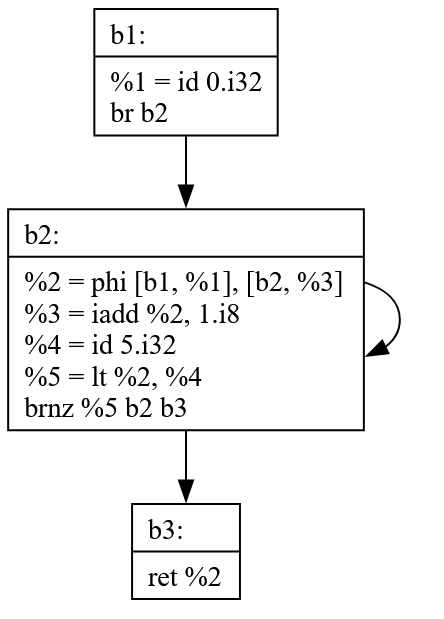
\includegraphics[scale=0.3]{images/i2.png}
\end{figure}

Next, after the \textit{PhiElim} pass is executed,
we can see that a critical edge must be broken, so the new \textit{crit\_0} block is created.

\begin{lstlisting}
  fn main() %0:i32
  b1:
    %1 = id 0.i32
    %302 = mov %1
    br b2
  crit_0:
    %302 = mov %3
    br b2
  b2:
    %2 = mov %302
    %3 = iadd %2, 1.i8
    %4 = id 5.i32
    %5 = lt %2, %4
    brnz %5 crit_0 b3
  b3:
    ret %2
\end{lstlisting}

\begin{figure}[H]
  \centering
  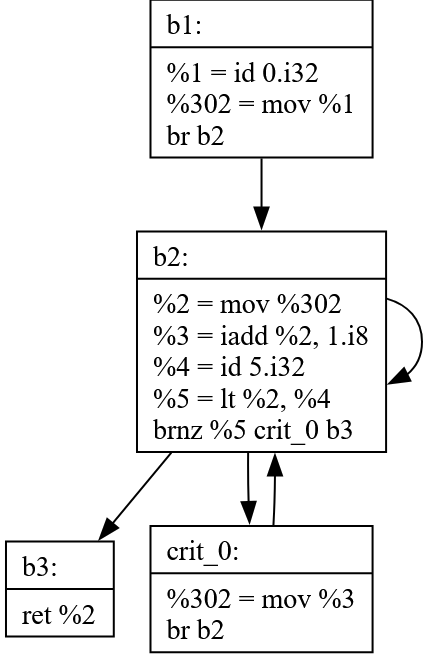
\includegraphics[scale=0.3]{images/i3.png}
\end{figure}

The phi node was successfully eliminated and replaced with \textit{mov} instructions,
so it can now easily be lowered to machine instructions and executed.
However, there is also one extra edge in the diagram above from \textit{b2} to itself although it's never possible to use it.
This shows that I'm not cleaning up dead edges properly somewhere in one of my passes.
I most likely would not have noticed this if a visualization pass was not made, but now I found a small bug I can fix in a future week.

For completeness, here is a full end to end example going from initial JBIR to 64-bit x86 machine code, including register allocation.
This example is partially out of date now, a \textit{mov} would replace the \textit{noop} inserted in place of the \textit{phi} and it also relies on the partially working \textit{Mem2Reg} pass from last week.

Initial JBIR:
\begin{lstlisting}
  fn main() %0:i32
  entry:
    %1 = slot i32
    stack_store %1, 100.i8
    %3 = id 1.i32
    brnz %3 first second
  first:
    br last
  second:
    stack_store %1, 42.i8
    br last
  last:
    %5 = stack_load %1 i32
    ret %5
\end{lstlisting}

\begin{figure}[H]
  \centering
  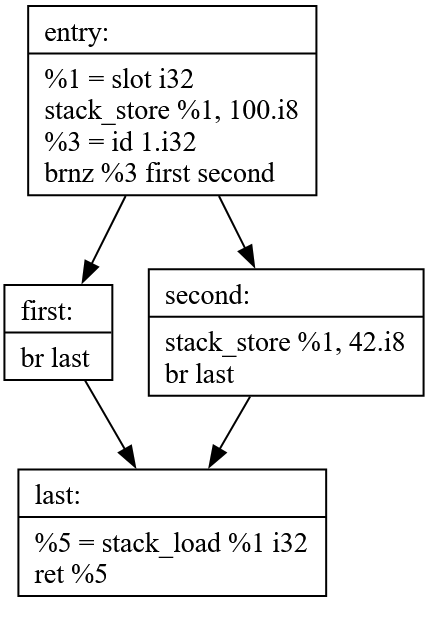
\includegraphics[scale=0.3]{images/i4.png}
\end{figure}

Resulting JBIR after the Mem2Reg pass is run.

\begin{lstlisting}
  fn main() %0:i32
  entry:
    noop
    %1000 = id 100.i8
    %3 = id 1.i32
    brnz %3 first second
  first:
    br last
  second:
    %1001 = id 42.i8
    br last
  last:
    %5 = phi [first, %1000], [second, %1001]
    ret %5
\end{lstlisting}

\begin{figure}[H]
  \centering
  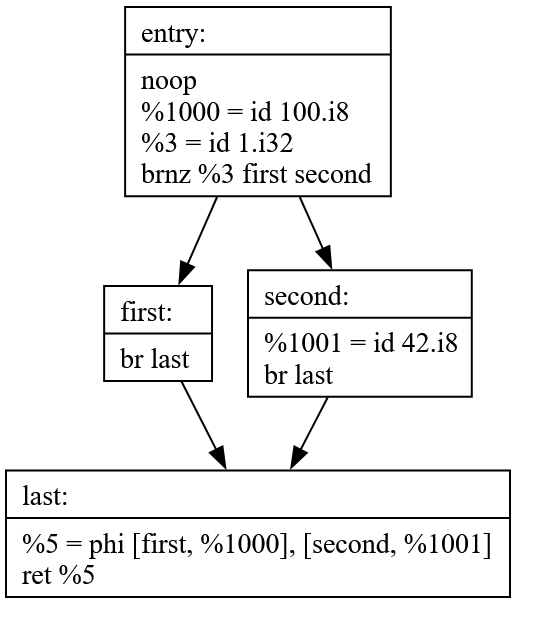
\includegraphics[scale=0.3]{images/i5.png}
\end{figure}

Resulting JBIR after \textit{PhiElim}.
\begin{lstlisting}
  fn main() %0:i32
  entry:
    noop
    %1000 = id 100.i8
    %3 = id 1.i32
    brnz %3 first second
  first:
    br last
    %5 = mov %1000,
  second:
    %1001 = id 42.i8
    br last
    %5 = mov %1001,
  last:
    noop
    ret %5
\end{lstlisting}

\begin{figure}[H]
  \centering
  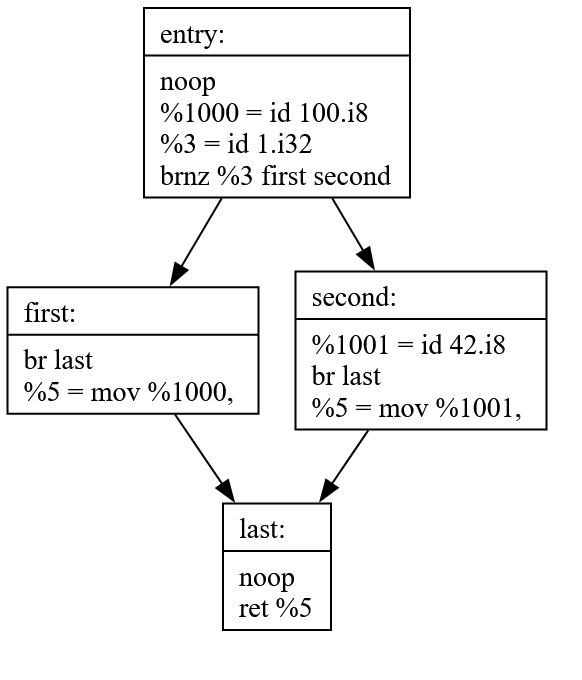
\includegraphics[scale=0.3]{images/i6.png}
\end{figure}

This is the MCIR, an internal compiler IR that's closer to the machine,
generated from the JBIR above.

\begin{lstlisting}

  main() %0:i32
  prolog:
    push %100:rbp
    mov %100, %101:rsp
    sub %101, 0
  entry:
    mov %1000, 100
    mov %3, 1
    cmp %3, 0
    jnz first
    jmp second
  first:
    jmp last
    mov %5, %1000
  second:
    mov %1001, 42
    jmp last
    mov %5, %1001
  last:
    mov %0, %5
    jmp main_exit
  main_exit:
    add %101, 0
    pop %100
    ret %0:rax
\end{lstlisting}

These are the live intervals for each virtual register.

\begin{lstlisting}
  0 | 14 18
  3 | 5 6
  5 | 10 14
100 | 1 17
101 | 2 16
1000 | 4 10
1001 | 11 13
\end{lstlisting}

Then, register allocation is done,
here is the output while iterating over live intervals and assigning/expiring registers.

\begin{lstlisting}
  [1,17] assigning a register: 100->5
  [2,16] assigning a register: 101->4
  [4,10] assigning a register: 1000->0
  [5,6] assigning a register: 3->1
  expired a register: 0
  expired a register: 1
  [10,14] assigning a register: 5->0
  [11,13] assigning a register: 1001->1
  expired a register: 0
  expired a register: 1
  [14,18] assigning a register: 0->0
\end{lstlisting}

Lastly, this is the final machine code after register allocation.

\begin{lstlisting}
  main() %0:i32
  prolog:
    push $rbp
    mov $rbp, $rsp
    sub $rsp, 0
  entry:
    mov $rax, 100
    mov $rcx, 1
    cmp $rcx, 0
    jnz first
    jmp second
  first:
    jmp last
    mov $rax, $rax
  second:
    mov $rcx, 42
    jmp last
    mov $rax, $rcx
  last:
    mov $rax, $rax
    jmp main_exit
  main_exit:
    add $rsp, 0
    pop $rbp
    ret $rax
\end{lstlisting}

\subsection{Week 4}

The implementation activities for this week were the Sparse Simple Constant Propagation(SSCP) and Dead Code Elimination(DCE) optimization passes.

First, an example of the DCE pass. The entry node for this function is b1, so the b2 block is dead, there's no possible way to reach it during normal program flow.

\begin{figure}[H]
  \centering
  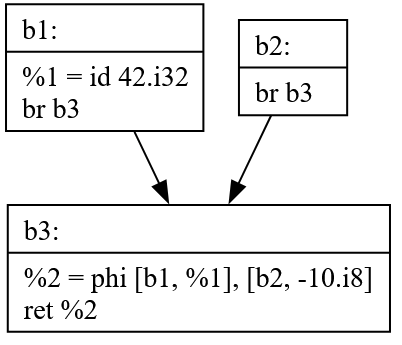
\includegraphics[scale=0.3]{images/i7.png}
\end{figure}

After running the DCE pass, we can see that it indeed found the \textit{b2} block to be dead as well, and removed it.

\begin{figure}[H]
  \centering
  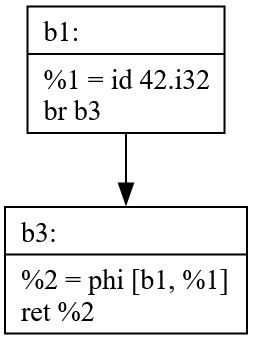
\includegraphics[scale=0.3]{images/i8.png}
\end{figure}

Next, an example of the SSCP pass, here is the original IR. All the instructions operate on constants so there's no need to execute these at runtime.

\begin{figure}[H]
  \centering
  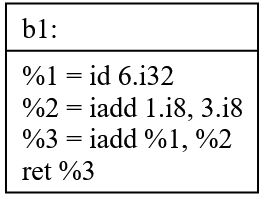
\includegraphics[scale=0.3]{images/i9.png}
\end{figure}

Then, the IR after running the SSCP Pass. As you can see, all the constant operations have been folded and it's just a ret with a constant.

\begin{figure}[H]
  \centering
  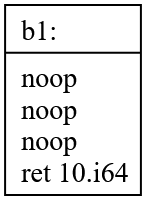
\includegraphics[scale=0.3]{images/i10.png}
\end{figure}

Now let's look at a full example that relies on both passes working correctly.
Here is the original IR.

\begin{figure}[H]
  \centering
  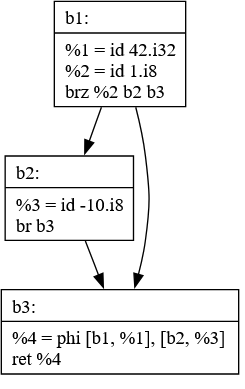
\includegraphics[scale=0.3]{images/i11.png}
\end{figure}

The first pass we run is the SSCP pass,
since there are no dead blocks yet so DCE would essentially be a \textit{noop}.
Lucky for us, SSCP basically folds all the instructions in \textit{b1} and \textit{b2} into the \textit{phi} in \textit{b3}.
Here is the IR after running SSCP.

\begin{figure}[H]
  \centering
  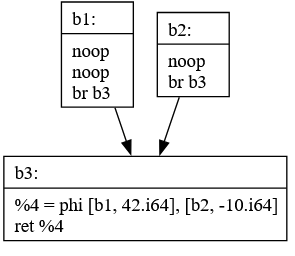
\includegraphics[scale=0.3]{images/i12.png}
\end{figure}

Now we have a familiar situation, with a dead b2 block, so DCE should be run, which results in the following.

\begin{figure}[H]
  \centering
  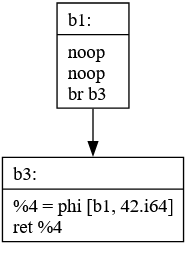
\includegraphics[scale=0.3]{images/i13.png}
\end{figure}

Running another round of SSCP then a version of the "Clean" algorithm mentioned in the book, to cleanup the CFG, would bring this down to a single ret instruction. The "Clean" algorithm simply cleans up the CFG and removes uncessary basic blocks, branches, edges, etc.

Some features I plan to work on in future works are a JBIR generator for the frontend so that I can generate JBIR directly from C instead of manually constructing it, a dominance analysis pass, fixing the Mem2Reg pass so it uses dominance information, a peephole/pattern-matching pass to catch simple identities(x*0=0, x+0=x, etc.), and a MergeExit pass for ensuring each function has a unique exit node.

\subsection{Week 5}

This is the first week where there's no assigned implementation activity, so I get to pick. I decided the most impactful feature to work on overall was a JBIR generator for the C frontend(JCC). This will make creating realistic examples much easier since I won't have to manually construct the IR anymore. It will also allow me to test my compiler on "real code" after the frontend gets to a point where it can parse the main features of C effectively.

Taking inspiration from the LLVM generator I made previously for JCC I worked on the JBIR one,and I can now generate JBIR directly from the C frontend.
It passes 81/94 of my test cases when using the interpreted backend(x86\_64 still needs some work), 
for comparison the LLVM version passes all available test cases.
I ended up having to add 6 more IR Ops to JBIR, mostly binary ops like \textit{and}, \textit{or}, \textit{xor}, \textit{left shift}, and \textit{right shift}.
The main features that cause the remaining failing tests are \textit{store}/\textit{load} from arbitrary pointers(not local variable),
aggregate types, and string literals(global/static data).
A major blocker for running the native backend is that the x86\_64 backend in JB still lacks support for a few instructions,
\textit{cmp} being the most inconvenient one, so it can only run a subset of tests that work in the interpreted backend.
Also, having the functionality to generate JBIR has already greatly simplified the process of creating more complex test/examples.
I already found plenty of cases where normal-looking C code breaks the \textit{Mem2Reg} pass, which is helpful.

Here is a simple example of a loop in C that can be parsed by JCC.

\begin{lstlisting}
  int main() {
    int a = 0;
  
    for(int i = 0; i < 10; i++) {
      if(i % 2 == 0)
        a += i;
      else
        a -= 1;
    }
  
    return a;
  }
\end{lstlisting}

JCC generates the following JBIR for the C code above.
This ends up producing the expected results when executed by JB, which is a big milestone!

\begin{figure}[H]
  \centering
  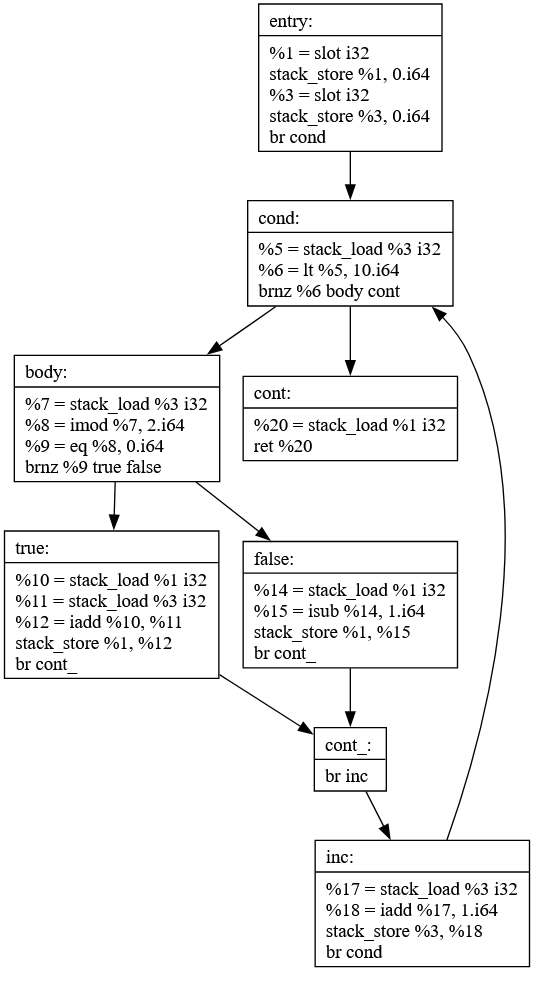
\includegraphics[scale=0.4]{images/i14.png}
\end{figure}

Here is the C code for another example I worked on that I found caused some incorrect behavior.
After investigating, I found my mistake to be incorrectly handling naming for the fallthrough/then block.
The fix was just making sure I did not accidentally create two blocks with the same name,
so instead I would create a block called \textit{cont\_} if "cont" already exists. 

\begin{lstlisting}
  int main() {
    int a = 20;
  
    if(a < 50) {
      if(a > 25) {
        a = 26;
      } else {
        a = 24;
      }
    } else {
      a = 1000;
    }
  
    return a;
  }
\end{lstlisting}

This is the corresponding JBIR for the C code above. As you can see, I made sure the names are not accidentally the same by appending an underscore where necessary, additionally two underscores would be appended if that were to clash with an existing name as well.

\begin{figure}[H]
  \centering
  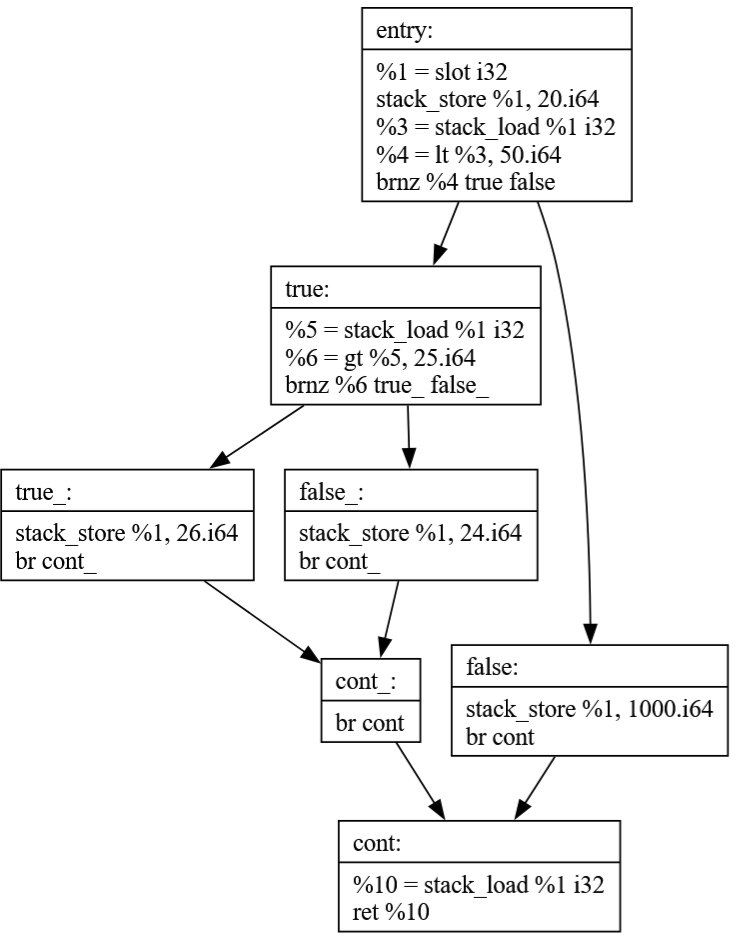
\includegraphics[scale=0.4]{images/i15.png}
\end{figure}

Just for fun I decided to run my Mem2Reg pass on this as well, even though it's not fully correct I know this is a case it will handle fine. In a future week, after dominance analysis is done, I'll fix this pass.

\begin{figure}[H]
  \centering
  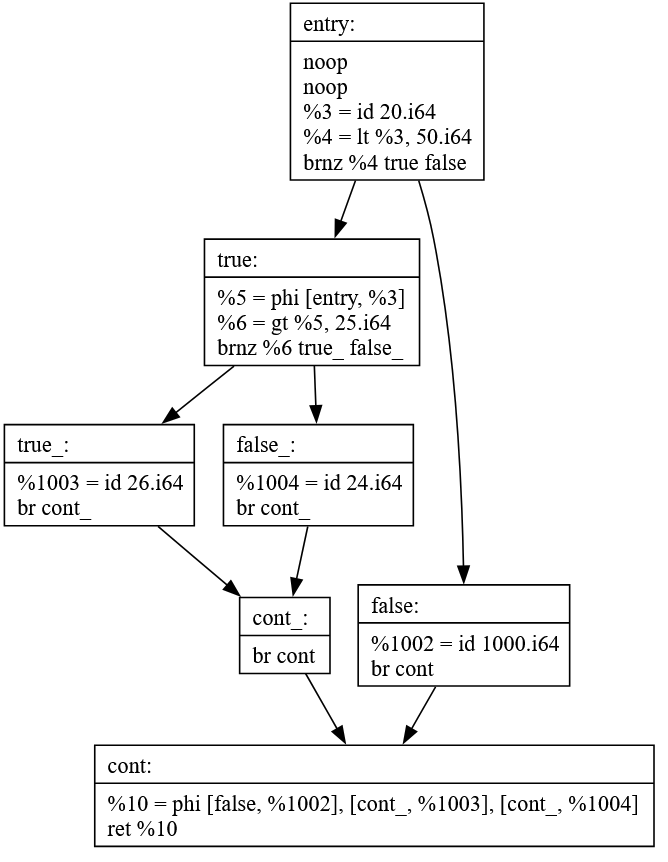
\includegraphics[scale=0.4]{images/i16.png}
\end{figure}

\subsection{Week 6}

For this week the implementation activity was Global Value Numbering (GVN). The first issue I ran into was that I didn't have a way to traverse the dominator tree because it was not implemented yet. As a result I couldn't rely on phi operands having value numbers already. In other words, I may visit a block without first visiting all it's dominators, so I may not have seen the definitions of it's operands yet. The easy "suboptimal" workaround is to give all phi targets a new value number, instead of potentially using a value number from an operand when possible, which is what I did for now. I could have also checked if all operands had numbers assigned then continue with the "optimal" version if so, but I figured I might as well start implementing a dominator tree and skip the problem entirely. Therefore, I decided to implement the easy dominance algorithm shown below. Unfortunately, it infinite loops on some inputs and also an "unpacking step" still needs to be done to make it usable for traversing over the dominator tree.

\begin{figure}[H]
  \centering
  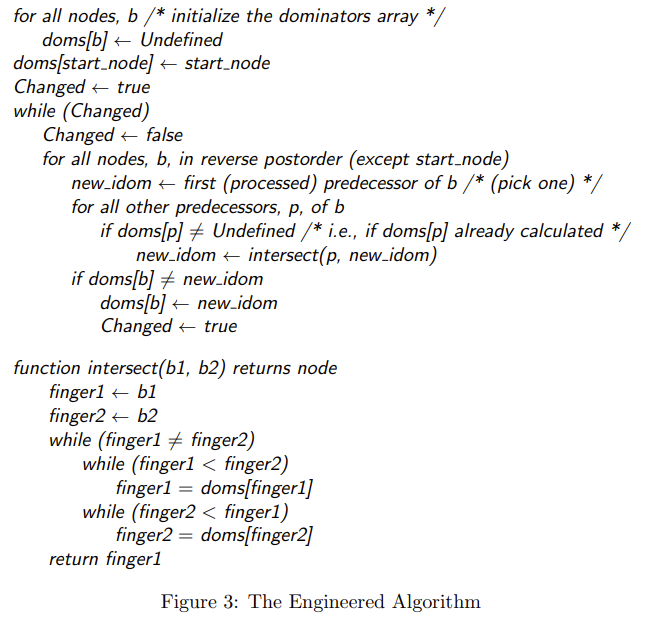
\includegraphics[scale=0.4]{images/i17.png}
\end{figure}

The dominator-based value numbering algorithm using hashing is an extension of the technique used for the value-numbering algorithm I already implemented. As a result, it shouldn't be too hard to adapt it in the future.

Here is a small example of the new Global Value Numbering(GVN) pass. The original JBIR is below.

\begin{figure}[H]
  \centering
  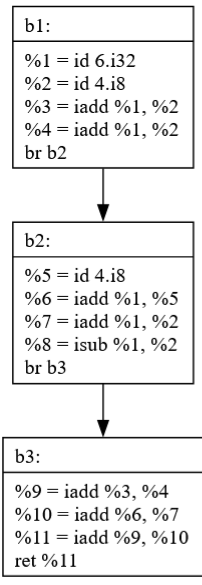
\includegraphics[scale=0.3]{images/i18.png}
\end{figure}

After running GVN, the IR below is the result. Also, as explained previously, it does not handle phi instructions "optimally" so I didn't include more complex control flow in this example.

\begin{figure}[H]
  \centering
  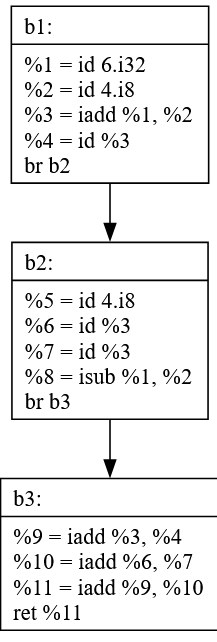
\includegraphics[scale=0.3]{images/i19.png}
\end{figure}

GVN can't do anything else for this example, but since the original operands were constants anyways SSCP would have folded everything regardless. The IR below is the result of running SSCP just for fun. I could also run a CFG cleanup pass and it would fully fold it to a single ret.

\begin{figure}[H]
  \centering
  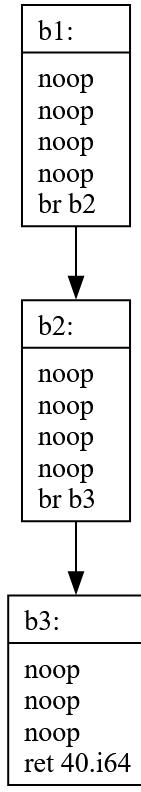
\includegraphics[scale=0.3]{images/i20.png}
\end{figure}

\subsection{Week 7}

For this week, the goal was to implement a peephole optimization pass. Overall, this was a relatively simple pass to implement compared to the previous few weeks, but it's still important. Also, it feels like a good portion of the peephole pass would fit directly into SSCP instead of being separate. Regardless, I'm going to keep it separate though, especially since more complicated patterns can be added later and it can potentially be expanded to handle more complicated patterns.

I also started making a CFG/general cleanup pass similar to what has been mentioned in previous weeks. This will just help with removing blocks that only contain unconditional or constant branches and other similar transformations.

The following example uses a non-constant function argument \textit{\%0} to showcase that these transformations extend what was previously possible with the preexisting SSCP pass. Here is the original IR.

\begin{figure}[H]
  \centering
  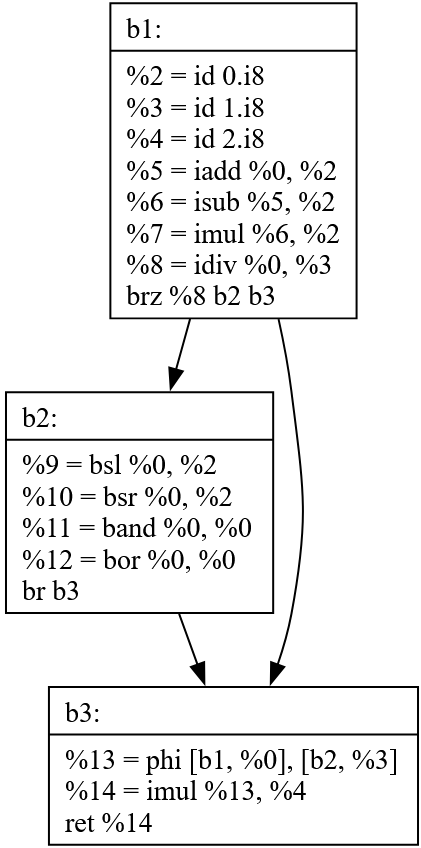
\includegraphics[scale=0.3]{images/i21.png}
\end{figure}

Running SSCP results in the following IR.

\begin{figure}[H]
  \centering
  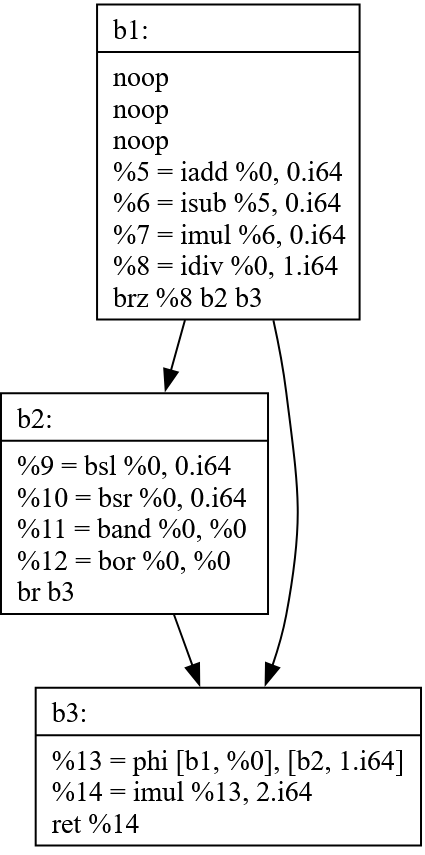
\includegraphics[scale=0.3]{images/i22.png}
\end{figure}

There were some instructions that SSCP wasn't able to do much with, so now the peephole pass is ran to hopefully take advantage of some algebraic identities.

\begin{figure}[H]
  \centering
  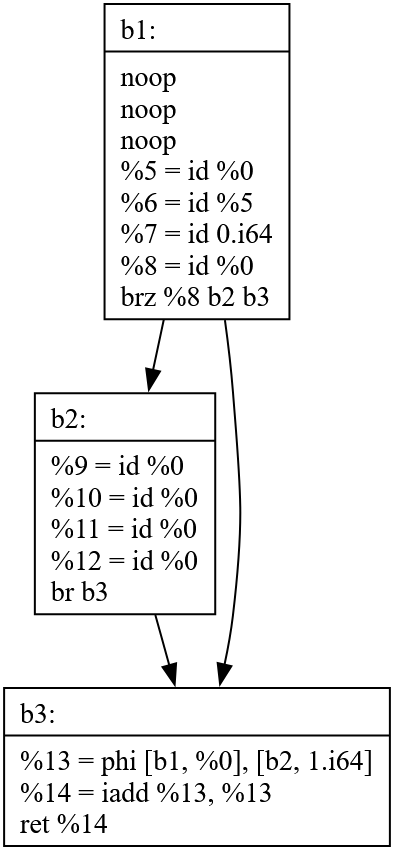
\includegraphics[scale=0.3]{images/i23.png}
\end{figure}

\subsection{Week 8}

Originally, the assigned implementation activity for this week was induction variable optimization, and although this type of optimization is useful there are some other optimizations in this section that have much higher potential benefit, not only from a performance standpoint but a learning one as well. As a result, I switched the implementation activity to instead be Loop-Invariant Code Motion(LICM). This is not a type of optimization that's often done on it's own and usually it is handled as part of a more general Lazy Code Motion(LCM). For that reason, I had created my own simple version of LICM, so I ended up implementing a version of what's described in the paragraph below.

A potential easy way to detect loop-invariant instructions would be by checking if all operands of an instruction in the loop body are themselves defined outside of the loop. This approach will be inefficient, but for each loop a pass can be done over the whole function which marks all SSA definitions that appear outside/inside of the loop. Then I can iterate through all operands used in the loop and mark instructions as loop-invariant or not using the criteria above. Lastly, I would have to handle pulling those instructions into a block before the loop header. There will most likely be some extra complications that will arise with nested loops that must be handled.

The first step I did was adding loop annotations to basic blocks.
This allowed me to sidestep the complexity of loop detection since the frontend will always generate the annotations correctly.
Each loop is given an associated loop\_id by the frontend.
Additionally, a canonical loop will have the following basic blocks: entry, cond, body, inc, and exit.

Next I tried to break down this algorithm further so I can implement it effectively. Intuitively, I need to first find all loop-invariant SSA definitions. Then, all those definitions must be moved into the entry block of the loop, so they are only executed once. However, this uncovers an issue, if the loop never executes we are now executing statements that would have never happened before. To fix this, I need to evaluate the condition of the loop once, then execute all invariant statements. After that the normal loop can then be executed, but the loop condition for the first iteration should not be evaluated again. Essentially, I want to transform all loops into the structure "if(cond) { do {} while(cond) }". Separating this into a loop transformation pass that automatically converts all loops to the structure described would probably be good. Especially since I can see this being useful elsewhere in the compiler. Also, at the moment, since this transforms loops into a non-canonical form, it destroys the usefulness of all loop annotations on basic blocks.

I ended up implementing two algorithms, the first being very simple but then I noticed it can accidentally move code into a path where it would not have been executed previously as explained above. The second algorithm handles the case described though.

A high-level overview of Algorithm 1: Move the invariant definitions up into the entry block. Then it needs to be ensured wherever a definition is moved, it's operands are available

A high-level overview of Algorithm 2: Create an invariant block.
Move instructions from old location into invariant block.
Add the invariant block after the cond block in the blocks list.
Then make cond jump to the invariant block or the exit block depending on it's condition.
After that, add a duplicate of the cond block, cond\_dup, after inc,
and make it jump to the body.
Lastly, make inc jump to the new cond\_dup block.

Next, I will show a small example to motivate the usefulness of this new pass. I will use a loop that finds the sum of numbers in range [0. 10), then adds 20 at the end. The 20 is calculated in the loop body, but is invariant, and the end result should be 65. Here is the equivalent C code that would do what is described. I should note, that while the frontend parse this correctly I am no using the IR it generates because it uses too many memory operations, these are intended to be handled by a working Mem2Reg pass.

\begin{lstlisting}
  int main() {
    int a = 0, b = 0;
    int c1 = 15, c2 = 5;
  
    for(int i = 0; i < 10; ++i) {
      a += i;
      b = c1 + c2;
    }
  
    return a + b;
  }
\end{lstlisting}

Here is the resulting hand-generated JBIR equivalent for the C code above.

\begin{figure}[H]
  \centering
  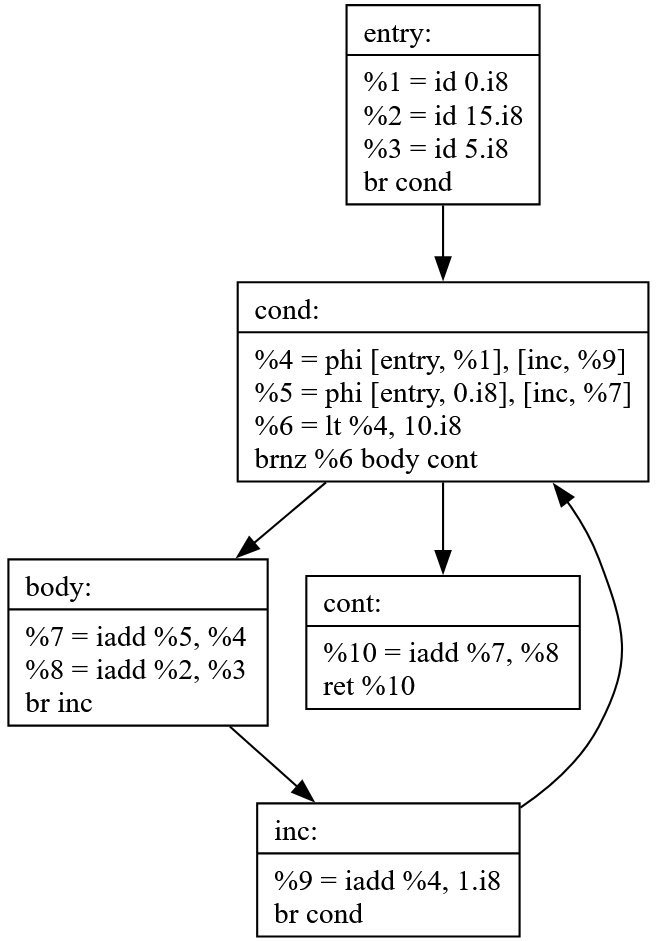
\includegraphics[scale=0.3]{images/i24.png}
\end{figure}

To get a better idea of what information the LICM pass looks for, here is the debug output it generates.

\begin{lstlisting}
  // List of all loops in function
  // format: (id: [list of blocks])
  1: entry, cond, body, inc, cont
  
  // All loop-independent ssa defs
  ind: 1, 10, 2, 3, 0, 8,
  
  // all loop-dependent ssa defs
  dep: 4, 5, 6, 7, 9,
  
  // All ssa defs located in the loop blocks
  defs: 1, 10, 2, 3, 0, 8,
  
  // intersection of ind and defs
  // printed as the actual instructions
  inv:    %8 = iadd %2, %3
\end{lstlisting}

This is the result after running Algorithm 1. While this transformation works in this example, as discussed earlier, a loop transformation needs to be done as well. If the loop condition is always false the loop-invariant code pulled into the entry block would never have executed previously, but now it does. This is not correct.

\begin{figure}[H]
  \centering
  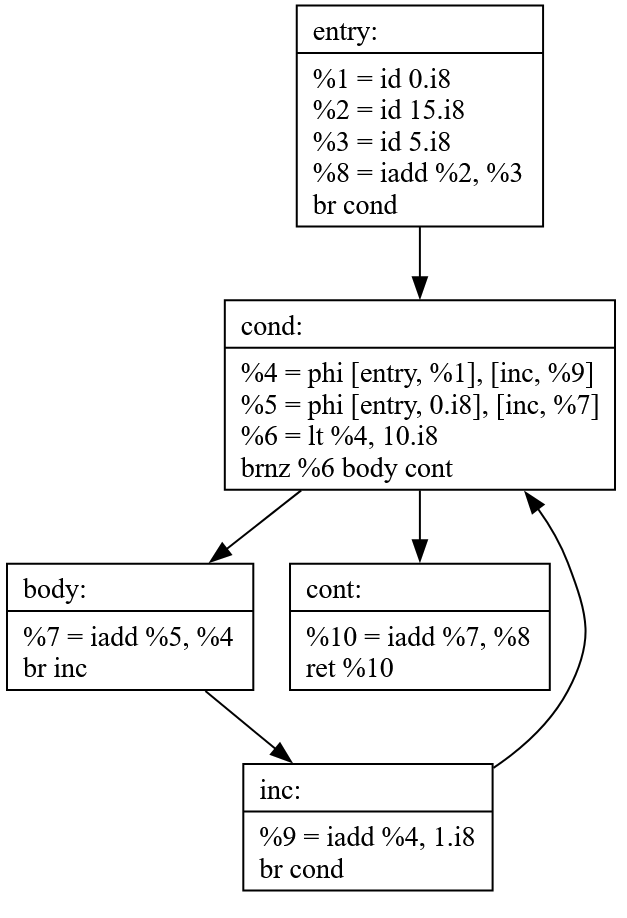
\includegraphics[scale=0.3]{images/i25.png}
\end{figure}

Now, this follows Algorithm 2 as outlined above to do the transformation. A note: some phi operands can be removed, this doesn't affect execution in the end though.

\begin{figure}[H]
  \centering
  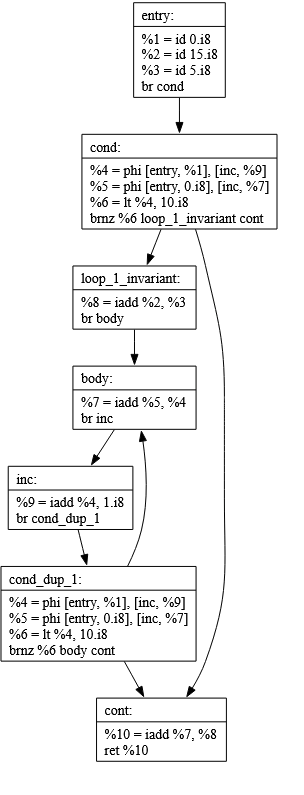
\includegraphics[scale=0.4]{images/i26.png}
\end{figure}

As expected, $65$ is the result when executing the original IR and the version where LICM is ran.

\subsection{Week 9}

This week the assigned activity was to implement a basic version of inlining.
Inlining is one of the most profitable optimizations, so it was very fun creating a simple working version.
I also continued implementing the basic CFG cleanup pass, so it now works good enough to be effective.
Additionally, there are some interesting problems regarding heuristics in this space that were not explored,
and instead functions are marked as "always\_inline" or not which helps to make implementing inlining manageable in a single week.

These are the steps I took for inlining a function call: First, deep copy the callee function. Second, rename all parameters, SSA names, and labels so they don't conflict. Third, space needs to be made for the function body, so the basic block containing the call instruction is split into two basic block around the call instruction. Fourth, copy all basic blocks from the function into the caller. Fifth, stitch the callee entry/exit blocks into the call site, in other words add the correct jumps in/out of the inlined function body so it is seamlessly intergrated into the caller. Lastly, the function parameters and return value must be put into the correct virtual registers, both the caller and calle expect these values to have different names just as a side effect of how these are handled in normal code.

Here is a simple example of a single add function.

\begin{lstlisting}
  int add(int lhs, int rhs) {
    return lhs + rhs;
  }
  
  int main() {
    return add(3, 39);
  }
\end{lstlisting}

This is the IR for the add and main functions respectively.

\begin{figure}[H]
  \centering
  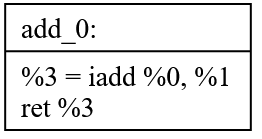
\includegraphics[scale=0.3]{images/i27.png}
  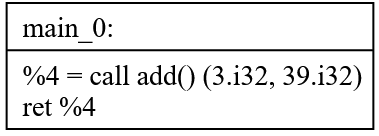
\includegraphics[scale=0.3]{images/i28.png}
\end{figure}

Here is the resulting IR of the main function after inlining. As expected the function body of add is copied and integrated directly into main.

\begin{figure}[H]
  \centering
  \includegraphics[scale=0.3]{images/i29.png}
\end{figure}

To further optimize this IR the cleanup pass and SSCP can be ran, here are the results of running those passes.

\begin{figure}[H]
  \centering
  \includegraphics[scale=0.3]{images/i30.png}
  \includegraphics[scale=0.3]{images/i31.png}
\end{figure}

The previous example was very simple, so I decided to see if my algorithm could work effectively on something a bit more complicated.
I took this example from the inlining wikipedia page \cite{inlinewiki}, and did some edits to allow for more optimizations to apply. 

Here is the equivalent C code for the example I'll be using. Assuming all optimizations work correctly, this would be folded down to just returning a single constant in main.

\begin{lstlisting}
  int pred(int x) {
    if (x == 0)
      return 0;
    else
      return x - 1;
  }

  int func(int y) {
    return pred(y-2) + pred(y+1) + pred(0);
  }

  int main() {
    return func(2);
  }
\end{lstlisting}

Also, this is the IR for the following functions in order: \textit{pred}, \textit{func}, and \textit{main}.

\begin{figure}[H]
  \centering
  \includegraphics[scale=0.3]{images/i32.png}
  \includegraphics[scale=0.3]{images/i33.png}
  \includegraphics[scale=0.3]{images/i34.png}
\end{figure}

After inlining everything into main the IR looks like the following.

\begin{figure}[H]
  \centering
  \includegraphics[scale=0.4]{images/i35.png}
\end{figure}

Then I ran the cleanup pass and SSCP.

\begin{figure}[H]
  \centering
  \includegraphics[scale=0.3]{images/i36.png}
  \includegraphics[scale=0.3]{images/i37.png}
\end{figure}

After that I ran Cleanup, SSCP, and DCE in a loop until no changes were left. Unfortunately though, something breaks eventually because phi instructions are not handled properly, so this will be something I fix in a future week.

\begin{figure}[H]
  \centering
  \includegraphics[scale=0.3]{images/i38.png}
\end{figure}

\subsection{Week 10}

There are no more assigned implementation activities for the rest of the study, so now I can focus on areas that will have the most impact. This week I decided to fix the bug I ran into during inlining last week. However, it didn't end up being a single bug and was instead a combination of multiple interacting mistakes. First, bug one was that when deep cloning a function the basic blocks in phi operands were replaced properly, but their values weren't, so for phi [[bb1, v1], [bb2, v2]] the v1 and v2 were not renamed properly and would instead be referring to values that don't exist in the current function. Second, bug two was simpler and in the interpreter, return values were overwritten during nested function calls. Lastly, bug three was fun, I accidentally used a brz instead of a brnz in the test case, so my conditions were flipped.

In a future week, one small thing I need to add is the ability to run sets of optimizations to a fixed point. To enable this, passes just need to report back whether they made changes or not and then I can decide whether or not to rerun them based on that. Also, I want to add a very simple heuristic for inlining, just something based on number of instructions and number of basic blocks in a function.

Using the same example from last week, here is the IR for the functions pred, func, and main respectively.

\begin{figure}[H]
  \centering
  \includegraphics[scale=0.3]{images/i39.png}
  \includegraphics[scale=0.3]{images/i40.png}
  \includegraphics[scale=0.3]{images/i41.png}
\end{figure}

After running inlining here is the IR for the following functions in order: pred, func, and main.

\begin{figure}[H]
  \centering
  \includegraphics[scale=0.3]{images/i42.png}
  \includegraphics[scale=0.3]{images/i43.png}
  \includegraphics[scale=0.3]{images/i44.png}
\end{figure}

Then I run SSCP, DCE, and Cleanup, as a group, to a fixedpoint, although manually for now which results in the following IR for pred, func, and main respectively. As expected main is able to be folded completely to just returning a single constant! The other two functions can not be folded on their own though, which is also expected. This is a big step for being able to effectively optimize more real-world programs, although it would be helpful if functions don't need to be explicitly marked for inlining and instead was done automatically using a heuristic.

\begin{figure}[H]
  \centering
  \includegraphics[scale=0.3]{images/i45.png}
  \includegraphics[scale=0.3]{images/i46.png}
  \includegraphics[scale=0.3]{images/i47.png}
\end{figure}

\subsection{Week 11}

Last week I was manually running passes until a fixed point, so this week I decided to work on pass management I made it automatic. Each pass now reports when it made a change and sets of passes can now be run until no more changes are made. There isn't much to show since the results of the example from last week are identical, just the implementation is different. Here is a sample of what the new pass management looks like.

\begin{lstlisting}
  bool changed;
  do {
    changed = false;
    changed |= SSCP::run_pass(f);
    CreateCFG::run_pass(f);
    CFGViz::run_pass(f);
  
    changed |= DCE::run_pass(f);
    CreateCFG::run_pass(f);
    CFGViz::run_pass(f);
  
    changed |= Cleanup::run_pass(f);
    CreateCFG::run_pass(f);
    CFGViz::run_pass(f);
  } while(changed);
\end{lstlisting}

Now I'll briefly lay out some potential next steps. Being able to register passes that should be run after/before certain types of passes or every pass would be cool, I wouldn't have to copy and paste visualization passes everywhere. Something else that would be helpful is creating a better optimization debug mode, especially with the combination of bugs I ran into a couple weeks ago. Basically something that would run the CFGViz pass after every pass and give an easy way to browse the changes made by each pass in the pipeline. Something like a simple html visualization. Running some "real" C projects is also something I've been meaning to try doing. The main blockers will most likely be frontend features though, which is the main reason I've been holding off(mainly the preprocessor). I'm sure I can find some examples that I could see benefit from optimizations I've written though. Also, another small pass I need to implement is the MergeExit pass which would just make each function have a single unique return/exit block. This ties in to general types of traversal over blocks of a function that is needed by other passes. Additionally, I want to spend a bit more time looking into loop optimizations and the polyhedral model. I'll try to fit some related topics into future weeks. Lastly, finishing the dominator tree implementation and fixing Mem2Reg has been something else I've been meaning do.

\subsection{Week 12}

Most of this week was spent reading the intel x86 manual to figure out how to encode instructions correctly.
This was because I added support for a bunch of new opcodes in the x86\_64 backend.
I finished implementing \textit{lt}, \textit{gt}, \textit{lte}, \textit{gte}, and \textit{eq}.
Then I also started implementing \textit{bsl}, \textit{bsr}, \textit{band}, \textit{bor}, and \textit{bxor}. Lastly, corresponding tests for all of the new instructions were added in JB.

\begin{table}[h!]
  \centering
  \begin{tabular}{|c|c|}
  \hline
  \textbf{JBIR Opcode} & \textbf{Meaning} \\
  \hline
  \hline
  lt & Less Than \\
  \hline
  gt & Greater Than \\
  \hline
  lte & Less Than or Equal \\
  \hline
  gte & Greater Than or Equal \\
  \hline
  eq & Equal \\
  \hline
  \end{tabular}
\end{table}
  
\subsection{Week 13}

First, I added support for more instructions in the x86\_64 backend.

\begin{table}[h!]
  \centering
  \begin{tabular}{|c|c|}
  \hline
  \textbf{JBIR Opcode} & \textbf{Meaning} \\
  \hline
  \hline
  bsl & Shift Left \\
  \hline
  bsr & Shift Right \\
  \hline
  band & Binary And \\
  \hline
  bor & Binary Or \\
  \hline
  bxor & Binary Xor \\
  \hline
  \end{tabular}
\end{table}

After that I started work on frontend support for arrays with the goal of being able to successfully compile/run the N-Queens solver below.
My initial strategy for array support was to desugar the array operation into pointer arithmetic during parse time, which I thought would be a quick change.
However, after implementing that, I realized that LLVM expects array operations to use a special GetElementPointer(GEP) instruction, so the "correct" way to implement array operations would be to keep them around explicitly in the AST for longer.
After finishing the LLVM implementation I will then move onto the JB one.

\begin{lstlisting}
  #include <stdbool.h>
  extern int printf(char*);
  
  int print_board(int board[][8]) {
    for (int i = 0; i < 8; i++) {
      for (int j = 0; j < 8; j++) {
        if (board[i][j])
          printf("Q ");
        else
          printf(". ");
      }
      printf("\n");
    }
    printf("\n\n");
  }
  
  bool conflict(int board[][8], int row, int col) {
    for (int i = 0; i < row; i++) {
      if (board[i][col])
        return true;
      int j = row - i;
      if (0 < col - j + 1)
        if (board[i][col - j])
          return true;
      if (col + j < 8)
        if (board[i][col + j])
          return true;
    }
    return false;
  }
  
  void solve(int board[][8], int row) {
    if (row == 8) {
      print_board(board);
      return;
    }
    for (int i = 0; i < 8; i++) {
      if (!conflict(board, row, i)) {
        board[row][i] = 1;
        solve(board, row + 1);
        board[row][i] = 0;
      }
    }
  }
  
  int main() {
    int board[64];
    for (int i = 0; i < 64; ++i) {
      board[i] = 0;
    }
    solve(board, 0);
  }
\end{lstlisting}

\subsection{Week 14}

This was a short week, only two days were not during fall break, so no notable implementation was finished.

\pagebreak
\section{Time Breakdown}

\begin{tabular}{ | c | c | }
    \hline
    Task & Hours Spent \\
    \hline
    \hline
    Reading (Engineering a Compiler) & $32.5$ \\
    \hline
    Reading (SSA Book) & $7$ \\
    \hline
    Reading (Misc.) & $33$ \\
    \hline
    Video & $8$ \\
    \hline
    Implementation & $72$ \\
    \hline
    Weekly Reports & $7.5$ \\
    \hline
    Final Report & $20.5$ \\
    \hline
    Meeting & $12$ \\
    \hline
    \hline
    Total & $192.5$ \\
    \hline
\end{tabular}

\pagebreak
\printbibliography

\end{document}